\documentclass[review]{elsarticle}

\usepackage{lineno,hyperref}
\modulolinenumbers[5]

\journal{Journal of \LaTeX\ Templates}

%%%%%%%%%%%%%%%%%%%%%%%
%% Elsevier bibliography styles
%%%%%%%%%%%%%%%%%%%%%%%
%% To change the style, put a % in front of the second line of the current style and
%% remove the % from the second line of the style you would like to use.
%%%%%%%%%%%%%%%%%%%%%%%

%% Numbered
%\bibliographystyle{model1-num-names}

%% Numbered without titles
%\bibliographystyle{model1a-num-names}

%% Harvard
%\bibliographystyle{model2-names.bst}\biboptions{authoryear}

%% Vancouver numbered
%\usepackage{numcompress}\bibliographystyle{model3-num-names}

%% Vancouver name/year
%\usepackage{numcompress}\bibliographystyle{model4-names}\biboptions{authoryear}

%% APA style
%\bibliographystyle{model5-names}\biboptions{authoryear}

%% AMA style
%\usepackage{numcompress}\bibliographystyle{model6-num-names}
\usepackage{amsmath}
\usepackage{psfrag}
\usepackage{graphicx}
\usepackage{epsfig}
\usepackage{epstopdf}
\usepackage{amssymb}



%% `Elsevier LaTeX' style
\bibliographystyle{elsarticle-num}
%%%%%%%%%%%%%%%%%%%%%%%

\newcommand{\paral}{\; \vert \;}
\newcommand{\myvec}[1]{\overrightarrow{#1}}
\newcommand{\Defeq}{\stackrel{\mathrm{df}}{=}}
\newcommand{\Bnfeq}{::=}
\newcommand{\Co}[1]{\overline{#1}}

%
\newcommand{\Bsep}{\: \mid \: }
\newcommand{\Rule}[2]{\displaystyle{\frac{#1}{#2}}}
\newcommand{\SF}[1]{\mathsf{#1}}
\newcommand{\Act}{\mathsf{Act}}
\newcommand{\Vis}{\mathsf{Vis}}
\newcommand{\ActK}{\mathsf{ActK}}
\newcommand{\Proc}{\mathsf{Proc}}
\newcommand{\Procc}{\mathsf{ProcC}}
\newcommand{\Pred}{\mathsf{Pred}}
\newcommand{\Std}{\mathsf{Std}}
\newcommand{\rms}{\mathrm{S}}
\newcommand{\rmrec}{\mathrm{rec}}
\newcommand{\rmreck}{\mathrm{reck}}
\newcommand{\rmreckR}{\mathrm{reckR}}
\newcommand{\rma}{\mathrm{A}}
\newcommand{\rmp}{\mathrm{P}}
\newcommand{\rmf}{\mathrm{F}}
\newcommand{\rmr}{\mathrm{R}}
\newcommand{\rmfr}{\mathrm{FR}}
\newcommand{\equivS}{\equiv_{\mathrm{S}}}
\newcommand{\SigSA}{\Sigma_{\mathrm{SA}}}
\newcommand{\ltran}[1]{\stackrel{#1}{\longrightarrow}}
\newcommand{\tran}[1]{\stackrel{#1}{\rightarrow}}
\newcommand{\nottran}[1]{\stackrel{#1}{\not\rightarrow}}
\newcommand{\Rtran}[1]{\stackrel{#1}{\rightsquigarrow}}
\newcommand{\notRtran}[1]{\stackrel{#1}{\not\rightsquigarrow}}
\newcommand{\trans}[1]{\stackrel{#1}{\rightarrow}_{\mathrm{S}}}
\newcommand{\Par}{\mid}
\newcommand{\restrict}[1]{\!\setminus\!#1}

\newcommand{\mA}{\mathcal{A}}
\newcommand{\mSA}{\mathcal{SA}}
\newcommand{\mWA}{\mathcal{WA}}
\newcommand{\mAK}{\mathcal{AK}}
\newcommand{\aAK}{\mathcal{(A)K}}
\newcommand{\umAK}{\underline{\mathcal{A}}\mathcal{K}}
\newcommand{\un}[1]{\underline {#1}}
\newcommand{\PI}{\mathcal{PI}}
\newcommand{\rom}[1]{\mbox{\rm{#1}}}

\newcommand{\Nil}{\mathbf{0}}
\newcommand{\New}[1]{\nu#1\: }
\newcommand{\Str}{\equiv}
\newcommand{\stdpred}{\mathsf{std}}
\newcommand{\std}[1]{\mathsf{std}(#1)}
%
\newcommand{\Bch}[2]{\mathsf{before}_{#1}(#2)}

\newcommand{\keys}[1]{\mathsf{keys}(#1)}
\newcommand{\kkey}[1]{\mathsf{k}(#1)}
\newcommand{\key}[1]{[#1]}
\newcommand{\Keys}{\mathcal{K}}
\newcommand{\freshpred}[1]{\mathsf{fsh}[#1]}
\newcommand{\fresh}[2]{\mathsf{fsh}[#1](#2)}

\newcommand{\ta}[1]{\mathsf{ta}(#1)}
\newcommand{\action}[1]{\mathsf{act}(#1)}

\newcommand{\intr}{\mbox{\ $\hat{}$\ }}
%\newcommand{\intr}{\mbox{\; $\widehat{}$\;}}
\newcommand{\sterm}{\mathsf{trm}}
\newcommand{\Sterm}[1]{\sterm(#1)}
\newcommand{\und}[1]{\underline{#1}}
\newcommand{\sqc}{\mathop{\cdot}}
\newcommand{\card}[1]{|#1|}
\newcommand{\bydef}{\stackrel{\emph{def}}{=}}
%
\newcommand{\Angle}[1]{\langle #1 \rangle}
\newcommand{\Tri}{\triangleright}
\newcommand{\hole}{\bullet}
\newcommand{\rec}[1]{\mathrm{rec}\, #1}
\newcommand{\Rec}[1]{\rec #1 .}
\newcommand{\Rch}{\mathsf{Rch}}
\newcommand{\prune}{\pi}
\newcommand{\Prune}[1]{\prune(#1)}
\newcommand{\Root}[1]{\mathsf{rt}(#1)}

\newcommand{\Bis}{\sim}
\newcommand{\Biss}{\Bis_{\mathsf{S}}}
\newcommand{\Bisf}{\Bis_{\mathsf{F}}}
\newcommand{\Bisfr}{\Bis_{\mathsf{FR}}}
%\newcommand{\Bisu}{\Bis_{\Un}}
\newcommand{\Sim}{\mathcal{S}}
\newcommand{\Rem}{\backslash}
\newcommand{\sqeqt}{\sim}
% rules:
% static rule
\newcommand{\one}{\mbox{(I)}}
\newcommand{\onef}{\mbox{(1)}}
\newcommand{\oner}{\mbox{(1R)}}
% choice rule
\newcommand{\two}{\mbox{(II)}}
\newcommand{\twof}{\mbox{(2)}}
\newcommand{\twor}{\mbox{(2R)}}
% choice axiom
\newcommand{\thr}{\mbox{(III)}}
\newcommand{\thrf}{\mbox{(3)}}
\newcommand{\thrr}{\mbox{(3R)}}
\newcommand{\thrpf}{\mbox{(3\,$'$\!)}}
\newcommand{\thrpr}{\mbox{(3\,$'$\!R)}}
%
%
\newcommand{\Draft}[1]{}
\newcommand{\Comment}[1]{}
\newcommand{\Rev}[1]{{#1}^{-1}}
\newcommand{\rulename}[1]{\textsf{#1}}

\newtheorem{theorem}{Theorem}
\newtheorem{definition}{Definition}
\newtheorem{remark}{Remark}
\newtheorem{example}{Example}
\newtheorem{proposition}{Proposition}


\begin{document}

\begin{frontmatter}

\title{Modelling and simulation of two gene repair pathways\tnoteref{mytitlenote}}
%\tnotetext[mytitlenote]{Fully documented templates are available in the elsarticle package on \href{http://www.ctan.org/tex-archive/macros/latex/contrib/elsarticle}{CTAN}.}

%% Group authors per affiliation:
\author{Stefan Kuhn}%\fnref{myfootnote}}
\address{School of Computer Science and Informatics, De Montfort University, Leicester, UK}
\ead{stefan.kuhn@dmu.ac.uk}
%\fntext[myfootnote]{Since 1880.}

\author{Irek Ulidowski}%\fnref{myfootnote}}
\address{School of Informatics, University of Leicester, Leicester, UK}
\ead{iu3@leicester.ac.uk}

%\fntext[myfootnote]{Since 1880.}
%% or include affiliations in footnotes:
%\author[mymainaddress,mysecondaryaddress]{Elsevier Inc}
%\ead[url]{www.elsevier.com}

%\author[mysecondaryaddress]{Global Customer Service\corref{mycorrespondingauthor}}
%\cortext[mycorrespondingauthor]{Corresponding author}
%\ead{support@elsevier.com}
%
%\address[mymainaddress]{1600 John F Kennedy Boulevard, Philadelphia}
%\address[mysecondaryaddress]{360 Park Avenue South, New York}

\begin{abstract}
We have demonstrated in previous work that the Calculus of Covalent Bonding (CCB) can be used to simulate higher-level biochemical processes. This is significant since CCB was originally devised to model organic chemical reactions on a lower level. We are now extending the use of CCB to model another gene repair pathway, DNA Mismatch Repair (MMR). This is a more complex pathway than the Base Excision Repair (BER) which we modelled originally. It involves four proteins and needs a distinction between the two chains in a DNA strand. We demonstrate that we can model this by extending our modelling of BER and that we can do this using the unchanged CCB calculus and operational semantics. We also show that the simulation software developed previously can be used to execute this pathway.
\end{abstract}

\begin{keyword}
%\texttt{elsarticle.cls}\sep \LaTeX\sep Elsevier \sep template
%\MSC[2010] 00-01\sep  99-00
\end{keyword}

\end{frontmatter}

\linenumbers

\section{Introduction}
Probably write this last, once we have the rest

\section{A Calculus of Covalent Bonding}\label{sec:calculus}

This is from socp paper, needs reworking

In this section we define the calculus introduced informally in the Introduction. 
First, we introduce some preliminary notions and notations.

Let $\mA$ be the set of (forward) action labels, 
ranged over by $a,b,c,d,e,f$. We partition $\mA$ into the set of \emph{strong actions}, written as
$\mSA$, and the set of \emph{weak actions}, written as $\mWA$. Reverse (or past) action labels are members of
$\underline\mA$, with typical members $\un{a},\un b, \un c,\un d, \un e ,\un f$, and represent 
undoing of actions. The set $\mathcal{P}(\mA \cup \underline\mA)$ is ranged over by $L$.

Let $\Keys$ be an infinite set of {\em communication keys} (or {\em keys} for short)
\cite{PhillipsUlidowski06,Irek2007}, ranged over by $k,l, m,n$. The Cartesian product $\mathcal A \times \Keys$, denoted by $\mAK$,
 represents past actions, which are written as $a[k]$ for $a\in \mA$ and $k\in\Keys$. 
Correspondingly, we have the set $\umAK$ that represents undoing of past actions. We use $\alpha, \beta$ to identify actions which are either from $\mA$ or $\mAK$. It would be 
useful to consider sequences of actions or past actions, namely the elements of $(\mA \cup \mAK)^*$, 
which are ranged over by $s,s'$ and sequences of purely past actions, namely the elements of $\mAK^*$, 
which are ranged over by $t,t'$. The empty sequence is denoted by $\epsilon$. We use the notation $\alpha, s$ and
$s,s'$ to denote a concatenation of elements, which can be strings or single actions.

We shall also use two sets of auxiliary action labels, namely the set $(\mA) =\{ (a)\ \mid a\in\mA\}$, and its product with the set of keys, namely $(\mA)\Keys$. These labels will be used in the auxiliary rules when defining
the semantics of CCB.

We now define the Calculus of Covalent Bonding, or CCB for short. The syntax of CCB is given 
below where $P$ is a process term:

$$P ::=  S \ \mid \ (s;b).P \ \mid \ P\paral Q \ \mid \ P\restrict L $$

The set of process identifiers (constants) $\PI$ contains typical elements $S$ and $T$. 
A process identifier $S$ has normally a defining equation $S\bydef P$ where $P$ contains only forward 
actions (and no past actions). There is also a special identifier
 $\Nil$, denoting the deadlocked process, which has no defining equation.

We have a general prefixing operator
$(s;b).P$, where $s$ is a non-empty sequence of actions or past actions. This operator
extends the prefixing operator in \cite{Irek2012}. The action $b$ is a weak action
and it can be omitted, in which case the prefixing is written as $(s).P$ and is called the
\emph{simple prefix}. The simple prefix is the prefixing operator in \cite{Irek2012}. 
One of the actions in $s$ in $(s).P$ may be a weak action from $\mWA$. If $s$ is a sequence that contains   
a single action, then the action is a strong action and the operator 
is the prefixing operator of CCS \cite{Milner1980}.
We omit trailing $\Nil$s so, for example, $(s).\Nil$ is written as $(s)$.
%
% Move this example to somewhere later
%
\Comment{\Stefan{We will only use cases in this paper where processes are of the form $(s).\Nil$. We still have the possibility of 
processes like $(s).(s').\Nil$ in our calculus. This could be used to model protein functions in biological systems, for example 
base excision repair (\cite{Koehler2014}. For this a protein ``walks'' along a strand of DNA and repairs faults which occurred in 
DNA replication. Such a protein could be modelled by having the walk modelled in $s$ and the repair mechanism in $s'$, combining them to a model like $(s).(s').\Nil$.}
}
%
%
The new feature of the operator $(s;b).P$ is the execution of the weak action $b$, which
can happen only after all the actions in $s$ have taken place. Performing $b$ then forces
undoing one of the past actions in $s$ (by the \rulename{concert} rule in Figure~\ref{fig:csos}).

$P\paral Q$ represents two systems $P$ and $Q$ which can perform actions or reverse actions on
their own, or which can interact with each other according to a communication function
$\gamma$. As in the calculus ACP \cite{ACPBook}, the communication function is a partial function 
$\gamma: \mathcal A \times \mathcal A \rightarrow \mathcal A$ which is commutative and associative. The function
$\gamma$ is used in the operational semantics to define when two processes can interact. Processes 
$P$ and $Q$ in $P\paral Q$ can also perform a pair of concerted actions,
which is the new feature of our calculus.  We also have the ACP-like restriction operator 
$\setminus L$, where $L$ is a set of labels. It prevents actions from taking place and, due to 
the synchronisation algebra used, it also blocks communication. If $\gamma(a,b)=c$ then $a.P$ and $b.Q$
cannot communicate in $(a.P\paral b.Q)\setminus c$.
Note that we do not use here the usual relabelling 
operator $[f]$, where $f: \mA \rightarrow \mA$, which could be easily added.

%
%move this elsewhere?
%
The example in the Introduction and our main example in Section~\ref{sec:bigexample} seem to indicate that only
simple processes of the form $(s;b).\Nil$ are sufficient in the modelling of chemical reactions. 
However, there are examples where a nested prefix $(s;b).(s';b').P$ is useful. 
Consider a base excision repair as in \cite{Koehler2014} where a protein ``walks'' along 
a strand of DNA and repairs faults which occurred in the DNA replication. The walking along a DNA strand 
could be modelled by actions in $s$, and, once a fault is found, the repair mechanism could be modelled
by the actions in $s'$. Another example where the full calculus is useful is a model of long 
standing transactions with compensations in \cite{Irek2012}.


The set of \emph{process terms} is ranged over by $P,Q$ and $R$ and is denoted by $\Proc$. 
In the setting of CCB these terms are called simply \emph{processes}. 
A context $C\hole$ is a process term containing a \emph{hole}, represented by $\hole$. 
Formally, contexts are defined by
the following syntax: $C::= \hole \mid (s;b).C \mid P\paral C \mid C \paral P \mid C\restrict L $.
The term $C[Q]$ denotes the result of filling the hole in the context $C\hole$ with the process $Q$.
We say that $R$ is a \emph{subprocess} of $P$ if $P$ is $C[R]$ for some context $C\hole$.

We define the semantics of our calculus by a labelled transition system,
LTS for short, which is a structure $(St,AL,\rightarrow: \subseteq St \times AL \times St)$
with $St$ the set of states, $AL$ the set of action labels and $\rightarrow: 
\subseteq St \times AL \times St$ the labelled transition relation.
The set of states $St$ is the set $\Proc$. In practice, all our results and examples hold for
\emph{consistent} processes, namely processes
reachable from standard processes (see Definition~\ref{consistent}). 
The action labels are the forward actions $\mAK$, 
the reverse actions $\umAK$ and the \emph{pairs of concerted actions} $\mAK \times \umAK$. 
%
The labelled transition relation is defined by SOS rules (Figures~\ref{fig:fsos}--\ref{fig:sc}) 
and rewrite rules (Figure~\ref{fig:reduction}), where
the rules in Figures~\ref{fig:fsos}--\ref{fig:reversesos}
are influenced by \cite{Irek2007}. 
Note that
sequences $s$ and $t$ are members of $(\mathcal{A}\cup\mathcal{AK})^*$ and $\mathcal{AK}^*$
respectively in Figures~\ref{fig:fsos}--\ref{fig:csos}.

We now introduce and explain the SOS rules before returning to 
the rewrite rules. Let $r$ be an SOS rule for an operator $f$ of CCB as in 
Figures~\ref{fig:fsos}--\ref{fig:csos}. 
%Then, $f$ is the operator of $r$ and the elements of $X$ are the arguments of $r$. 
%We write $rules(f)$ for the set of SOS rules for $f$. 
Transitions above the horizontal bar in $r$ are called \emph{premises}. 
The set of premises is written as
$pre(r)$. The transition below the bar in $r$ is the $\emph{conclusion}$ and 
is written as $con(r)$. 
%
\begin{figure}[t] 
\[
\begin{array}{ll}
\Rule
{}
{\std{\Nil}}
\qquad &
\Rule
{}
{\fresh{m}{\Nil}}
\\[15pt]
\Rule
{\std{P}}
{\std{S}}
\quad
S \bydef P
\qquad &
\Rule
{\fresh{m}{P}}
{\fresh{m}{S}}
\quad
S \bydef P
\\[15pt]
\Rule
{\kkey{s}=\emptyset \quad  \std{P}}
{\std{(s;b).P}}
\qquad &
\Rule
{m \notin \kkey{s} \quad \fresh{m}{P}}
{\fresh{m}{(s;b).P}}
\\[15pt]
\Rule
{\std{P} \quad \std{Q}}
{\std{P \paral Q}}
\qquad &
\Rule
{m \notin \kkey{s} \quad m \neq n \quad \fresh{m}{P}}
{\fresh{m}{(s;b[n]).P}}
\\[15pt]
\Rule
{\std{P}}
{\std{P \setminus L}}
\qquad &
\Rule
{\fresh{m}{P} \quad \fresh{m}{Q}}
{\fresh{m}{P \paral Q}}
\qquad 
\Rule
{\fresh{m}{P}}
{\fresh{m}{P \setminus L}}
\end{array}
\] 
\caption{Predicates $\mathsf{std}$ and $\mathsf{fsh}$.} 
\label{fig:predicates}
\end{figure}
%
We use two predicates $\std{P}:\Proc$ and $\fresh{m}{P}:\Keys \times \Proc$ in our SOS rules. 
They are defined in Figure~\ref{fig:predicates}, and they use two auxiliary functions
$\kkey{s}: (\mathcal{A}\cup\mathcal{AK})^* \rightarrow \mathcal{P}(\Keys)$ and
$\keys{P}: \Proc \rightarrow \mathcal{P}(\Keys)$. 
The function $\kkey$ is defined as follows:
$\kkey{\epsilon}=\emptyset$, $\kkey{\alpha:s}=\{l\}\cup\kkey{s} \text{ if }\alpha=a[l]$, for 
$a\in \mathcal{A}$ and $l\in \Keys$, and $\kkey{\alpha:s}= \kkey{s} \text{ if }\alpha \in \mathcal{A}$.
The function $\keys$ is given by $\keys{\Nil}=\emptyset$, $\keys{S}=\keys{P}$ if $S\bydef P$, $\keys{(s;b).
P}=\kkey{s} \cup \kkey{b} \cup \keys{P}$, $\keys{P \paral Q}= \keys{P} \cup \keys{Q}$, and $\keys{P \restrict L}=\keys{P}$. Informally $\keys{P}$ associates with each term $P$ the set of its keys. 
A process $P$ is standard, written $\std{P}$, if it contains no past actions (hence no keys). 
A key $n$ is fresh in $Q$, written $\freshpred{n}(Q)$, if $Q$ contains no past action with the key $n$.
We extend the notion of fresh keys to the sequences of actions and past actions $s$ and $t$ 
via the function $\kkey$.
%Figure~\ref{fig:predicates} defines the predicates by induction over the process terms. 
%We could also have said that $\std{P}$ is true if $\keys{P} = \emptyset$ and that 
%$\fresh{m}{P}$ is true if $i \notin \keys{P}$.

\begin{figure}[t] 
\[
\begin{array}{ll}
\rulename{act1}\ 
\Rule
{\std{P} \quad \fresh{k}{s,s'}}
{(s,a,s';b).P \xrightarrow{a[k]}(s,a[k],s';b).P}
\qquad &
\rulename{act2}\
\Rule
{P \xrightarrow{a[k]} P' \quad \fresh{k}{t}}
{(t;b).P \xrightarrow{a[k]} (t;b).P'}
\\[25pt]
%\rom{act3}\ Dec 17
%\Rule
%{\std{P} \quad \fresh{k}{t,t'}}
%{(t,b,t';b').P \xrightarrow{b[k]}(t,b[k],t';b').P}
%\qquad &
%\\[25pt]
\rulename{par}\
\Rule
{P \xrightarrow{a[k]} P'\quad \fresh{k}{Q}}
{P \paral Q \xrightarrow{a[k]} P' \paral Q}
\qquad &
\rulename{com}\
\Rule
{P \xrightarrow{a[k]} P' \quad Q \xrightarrow{d[k]} Q'}
{P \paral Q \xrightarrow{c[k]} P' \paral Q'}
\; (*)
%
\\[25pt]
\rulename{res}\
\Rule
{P \xrightarrow{a[k]} P'}
{P\backslash L \xrightarrow{a[k]} P'\backslash L}
\; a \notin L
\qquad &
\rulename{con}\
\Rule
{P \xrightarrow{a[k]} P'}
{S \xrightarrow{a[k]} P'}
\; S \bydef P
\end{array}
\] 
\caption{Forward SOS rules. The condition (*) is $\gamma(a,d)=c$, 
and $b \in \mathcal{WA}$.} \label{fig:fsos}
\end{figure}
\begin{example}
{\rm
We illustrate how processes compute forwards using the new prefixing operator. Consider a standard
process $(a;b).(c) \paral (a,d,c)$ and the communication function $\gamma$ given by $\gamma(a,a)=a$ 
and $\gamma(c,c)=c$. We have
$$(a;b).(c) \paral  (a,d,c) \xrightarrow{a[1]} (a[1];b).(c) \paral  (a[1],d,c)$$
by the SOS rules \rulename{act1} and \rulename{com} from Figure~\ref{fig:fsos}. This is because $(c)$ 
is standard and the key 1 is fresh in $\varepsilon$. The next step of computation involves a communication of
the actions $c$, which we obtain by rules \rulename{act2} and \rulename{com}:
$$(a[1];b).(c) \paral  (a[1],d,c) \xrightarrow{c[2]} (a[1];b).(c[2]) \paral  (a[1],d,c[2])$$
We note that the key 2 is fresh in $a[1]$. Finally, the action $d$ takes place by \rulename{act1} and,
informally, the symmetric version of \rulename{par}.
$$(a[1];b).(c[2]) \paral  (a[1],d,c[2]) \xrightarrow{d[3]} (a[1];b).(c[2]) \paral  (a[1],d[3],c[2])$$
Formally, we use \rulename{par}, the structural congruence rule \rulename{sc} in Figure~\ref{fig:sc}
and the reduction rule \rulename{red1} in Figure~\ref{fig:reduction}.
}
\end{example}

\begin{figure}[t]
\[
\begin{array}{ll}
\rulename{rev act1}\
\Rule
{\std{P} %\quad \fresh{k}{s,s'}
}
{(s,a[k],s';b).P \xrightarrow{\underline{a}[k]}(s,a,s';b).P}
\quad &
%
% b was previously beta. Since we must apply prom rewrite before we apply any SOS rule, we do not 
% need a rule with a beta.
%
% referees suggested to remove fsh predicates from both act rules. They were there for symmetry reason 
% with the forward rules but are not used in the reverse.
%
\rulename{rev act2}\
\Rule
{P \xrightarrow{\underline{a}[k]} P' %\quad \fresh{k}{t}
}
{(t;b).P \xrightarrow{\underline{a}[k]} (t;b).P'}
\\[25pt]
% Dec 17
%\rom{rev act3}\
%\Rule
%{\std{P}  \quad \fresh{k}{t,t'} }
%{(t,b[k],t';b').P \xrightarrow{\underline{b}[k]} (t,b,t';b').P'}
%& \\[25pt]
\rulename{rev par}\
\Rule
{P \xrightarrow{\underline{a}[k]} P'\quad \fresh{k}{Q}}
{P \paral Q \xrightarrow{\underline{a}[k]} P' \paral Q}
\quad &
\rulename{rev com}\
\Rule
{P \xrightarrow{\underline{a}[k]} P' \quad Q \xrightarrow{\underline{d}[k]} Q'}
{P \paral Q \xrightarrow{\underline{c}[k]} P' \paral Q'}
\; (*)
%
\\[25pt]
\rulename{rev res}\
\Rule
{P \xrightarrow{\underline{a}[k]} P'}
{P\backslash L \xrightarrow{\underline{a}[k]} P'\backslash L}
\; a \notin L
\quad &
\rulename{rev con}\
\Rule
{P \xrightarrow{\underline{a}[k]} P'}
{P \xrightarrow{\underline{a}[k]} S}
\; S \bydef P'
\end{array}
\]
\caption{Reverse SOS rules. The condition (*) is $\gamma(a,d)=c$, and 
and $b \in \mathcal{WA}$. %Note that $\beta \in \mA \cup \mAK$.
} 
\label{fig:reversesos}
\end{figure}

\begin{figure}[t] 
\[
\begin{array}{l}
\rulename{aux1}\ 
\Rule{\std{P} \quad \fresh{k}{t}}
{(t;b).P \xrightarrow{(b)[k]}(t;b[k]).P}
\qquad
\rulename{aux2}\
\Rule
{P \xrightarrow{(b)[k]} P' \quad \fresh{k}{t}}
{(t;b').P \xrightarrow{(b)[k]} (t;b').P'}
\\[25pt]
\rulename{concert}\ 
\Rule
{P\xrightarrow{(b)[k]}P' \quad P'\xrightarrow{\underline{a}[l]}P'' \qquad Q\xrightarrow{\alpha[k]}Q' 
  \quad Q'\xrightarrow{\underline{d}[l]}Q''% %\quad \fresh{k}{Q} 
 }
{P \paral Q\xrightarrow{\{e[k],\underline{f}[l]\}} P'' \paral Q''} (*)\\[25pt]
\rulename{concert act}\
\Rule
{P \xrightarrow{\{{a}[k], \underline{h}[l]\}} P' \quad \fresh{k}{t}}
{(t;b).P \xrightarrow{\{{a}[k], \underline{h}[l]\}} (t;b).P'}\\[25pt]
\rulename{concert par}\
\Rule
{P \xrightarrow{\{{a}[k], \underline{h}[l]\}} P'\quad \fresh{k}{Q} \quad \fresh{l}{Q}}
{P \paral Q \xrightarrow{\{{a}[k], \underline{h}[l]\}} P' \paral Q}\\[25pt]
\rulename{concert res}\
\Rule
{P \xrightarrow{\{{a}[k], \underline{h}[l]\}} P'}
{P\backslash L \xrightarrow{\{{a}[k], \underline{h}[l]\}} P'\backslash L} (**)
%
\end{array}
\] 
\caption{SOS rules for concerted actions. The condition (*) is 1. $\alpha$ is $c$ or $(c)$ 
and $\gamma(b,c)=e$ for some $c\in \mathcal{A}$, and 2. $\gamma(a,d)=f$. 
The condition (**) is $a, \underline{h}  \notin L \cup (L)$. 
Recall that $t \in \mAK^*$.} \label{fig:csos}
\end{figure}

\begin{figure}[t] 
\[
\begin{array}{l}
%\rom{sc}\
\Rule
{P \Rightarrow Q \quad Q \tran{\mu} Q' \quad Q' \Rightarrow P'}
{P\tran{\mu} P'} 
%\quad \mu \in \mAK\cup \umAK \cup \mathcal{C}
%%TODO Moreover, $S\equiv P$ for all $S, P$ 
%%such that $S\bydef P$.
\end{array}
\] 
\caption{Structural congruence rule sc when $\mu\in \mAK \cup (\mAK\times \umAK)$,
and rev sc when $\mu\in \umAK$.} 
\label{fig:sc}
\end{figure}

\begin{figure}[t] 
\[
\begin{array}{lll}
\rulename{red1}: & P\Par Q \Rightarrow Q\Par P& 
\\[10pt]
\rulename{red2}: & P\Par (Q\Par R) \Rightarrow (P\Par Q)\Par R &
\\[10pt]
\rulename{red3}: & (P\Par Q)\Par R \Rightarrow P\Par (Q\Par R) & 
\\[10pt]
\rulename{red4}: & P\Par \Nil \Rightarrow P & 
\\[10pt]
\rulename{red5}: & (P\paral Q)\backslash L \Rightarrow P\backslash L \paral Q & \mbox{ if fn(Q)} \cap L = \emptyset
\\[10pt]
\rulename{red6}: & P\backslash L \paral Q \Rightarrow (P\paral Q)\backslash L & \mbox{ if fn(Q)} \cap L = \emptyset
\\[10pt]
\rulename{prom}: & (s,a,s';b[k]).P \Rightarrow (s,a[k],s';b).P & \mbox{ if } a \in \mathcal{SA}, b \in \mathcal{WA} 
\\[10pt]
\rulename{move-r}: & (s,a,s',b[k],s'').P \Rightarrow (s,a[k],s',b,s'').P & \mbox{ if } a \in \mathcal{SA}, b \in \mathcal{WA}
\\[10pt]
\rulename{move-l}: & (s,b[k],s',a,s'').P \Rightarrow (s,b,s',a[k],s'').P & \mbox{ if } a \in \mathcal{SA}, b \in \mathcal{WA}
\end{array}
\] 
\caption{Reduction rules. Sequences $s, s', s''$ are members of $(\mathcal{A} \cup \mathcal{AK})^{*}$.} 
\label{fig:reduction}
\end{figure}

The next example illustrates how some of the reverse SOS rules work.
\begin{example}
{\rm 
Consider $(a[1],b).(c).S$ where $S\bydef (a,b).(c).S$. We have 
$$(a[1],b).(c).S \xrightarrow{\underline{a}[1]} (a,b).(c).S$$ by \rulename{rev act1} since $(c).S$ is standard.
Since $(a,b).(c).S$ is the definition of $S$ we obtain by rule \rulename{rev con} $(a[1],b).(c).S \xrightarrow{\underline{a}[1]} S$.
}
\end{example}

Figure \ref{fig:csos} contains the SOS rules that define the new concerted actions transitions. 
The main rule is the rule \rulename{concert} that defines when a pair of concerted actions 
takes place.  We also have two auxiliary rules \rulename{aux1} and \rulename{aux2} which 
define only an auxiliary transition relation needed in the \rulename{concert} rule. 
Note that the \rulename{concert} rule uses \emph{lookahead} \cite{Uli92}.
Also note that transitions in \rulename{aux1} and \rulename{aux2} use the auxiliary labels $(b)[k]$ 
for all $b \in \mWA$ and $k \in \Keys$. The rule \rulename{concert par} requires that $k$ is fresh in $Q$,
correspondingly as in \rulename{par}. Moreover, we need to ensure that when we reverse $h$ with the key $l$
in $P$ we do not leave out any actions with the key $l$ in $Q$ which make up a multiaction 
communication with the key $l$. Hence, we also include the premise $\fresh{l}{Q}$ in \rulename{concert par}.
The rule \rulename{concert act} requires, correspondingly as \rulename{act}, that $k$ is fresh in $t$.
Our operational semantics guarantees that if a standard process evolves to $(t;b).P$, for some $P$, and
$P$ reverses an action with the key $l$, then $l$ is fresh in $t$. Hence, we do not include $\fresh{l}{t}$
in the premises of \rulename{concert act}.
%
Next, we illustrate how concerted actions transitions work.

\begin{example}\label{ex:examp1}
{\rm Consider the process $(a;b) \paral a \paral b$ with $\gamma(a,a)=c$ and $\gamma(b,b)=d$. After the
initial synchronisation of actions $a$, which produces the transition $c[1]$, we have a transition
with a pair of concerted actions by rule \rulename{concert} in Figure~\ref{fig:csos}
$$(a[1];b) \paral a[1] \paral  b \xrightarrow{\{d[2], \underline{c}[1]\}} 
  (a;b[2])\paral a \paral b[2]$$
since $(a[1];b) \xrightarrow{(b)[2]} (a[1];b[2])$ by \rulename{aux1}, 
$(a[1];b[2]) \xrightarrow{\underline{a}[1]} (a;b[2])$ by \rulename{rev act1}, 
and since $a[1] \paral b \xrightarrow{b[2]} a[1] \paral b[2] \xrightarrow{\underline{a}[1]} a \paral b[2]$
by \rulename{par} and \rulename{rev par}.}
\end{example}

\begin{example}\label{ex:examp2}
{\rm Consider $(a[1];b)\paral (a[1];b)\paral e$ with $\gamma(a,a)=c$ and $\gamma(b,b)=d$.
We clearly have the following pair of concerted actions
 $$(a[1];b)\paral (a[1];b)\paral e  \xrightarrow{\{d[2], \underline{c}[1]\}} 
(a;b[2])\paral (a;b[2])\paral e. $$}
\end{example}

There are processes with weak actions that can potentially communicate but there are no concerted actions 
transitions due to our SOS rules:

\begin{example}\label{ex:examp3}
{\rm Consider $(a[1];b)\paral (e[2];b)\paral (a[1],e[2])$ with $\gamma(a,a)=c$ and $\gamma(b,b)=d$.
The process cannot perform any concerted actions: Although $(a[1];b)  \xrightarrow{(b)[l]} 
\xrightarrow{\underline{a}[1]} (a;b[l])$, for any $l$ different from 1 and 2, but
$(e[2];b)\paral (a[1],e[2])$  cannot perform the auxiliary $(b[l])$
transition since there are no SOS rules for parallel composition and auxiliary actions $(b)$. This forces us
to treat $(a[1];b)$ and $ (e[2];b)$ as $P$ and $Q$ in the \rulename{concert} rule, respectively, and we notice that
we cannot undo a communication on $a$ or $e$.}
\end{example}

Overall, the transitions in Figures~\ref{fig:fsos}--\ref{fig:csos} are labelled with $a[k] \in \mAK$, or with 
$\underline{c}[l] \in \umAK$, or with concerted actions $(a[k], \underline{c}[l])$.
%\} \in \mathcal{C}$.

We also have the usual structural congruence rules 
sc and rev sc in Figure~\ref{fig:sc}, 
which potentially combine reductions (defined below) with transitions.

Next, we introduce our reduction relation which is given by the reduction (rewrite) rules 
in Figure~\ref{fig:reduction}. The reduction relation is needed to define {\em promotion} 
of actions. First we define the function $\mathsf{fn}$ for {\em free names} of processes.

\begin{definition} \normalfont 
The function $\mathsf{fn}: \Proc \rightarrow \mathcal{P}(\Keys)$ is given as follows: 
$\mathsf{fn}(\Nil) = \emptyset$,
$\mathsf{fn}(S)=\mathsf{fn}(P) \text{ if }  S\bydef P$, $\mathsf{fn}((\alpha : s;b).P)=\{\alpha\} \cup 
\mathsf{fn}((s;b).P)$, $\mathsf{fn}((a;b).P)=\{a,b\} \cup \mathsf{fn}(P) $, $\mathsf{fn}(P\paral Q)=\mathsf{fn}(P) \cup \mathsf{fn}(Q)$, and $\mathsf{fn}(P \restrict L)=\mathsf{fn}(P) \restrict L$.
\end{definition}

\noindent
Our reduction rules have names such as, for example, \rulename{red} and we write 
\rulename{red}: $P \Rightarrow Q$
to indicate that the reduction rule $P \Rightarrow Q$ is called \rulename{red}. 
The process $P$ in the rule
$P\Rightarrow Q$ is called a \emph{redex}, and the process $Q$ is called a \emph{contractum}. 
A reduction rule $P\Rightarrow Q$ can be seen as a prescription 
for deriving rewrites $C[P] \Rightarrow C[Q]$ for arbitrary context $C[\ ]$. 
A $P$ redex may be replaced by its contractum $Q$ in an arbitrary context 
$C[\ ]$ giving rise to a reduction step: $C[P] \Rightarrow C[Q]$.

\begin{definition} \normalfont The reduction relation $\Rightarrow$ is the smallest reflexive and 
transitive relation on CCB processes that is preserved by all contexts, and that satisfies the rules 
in Figure~\ref{fig:reduction}.
\end{definition}
Note that we do not want $\Rightarrow$ to be symmetric as we wish to apply \rulename{prom} only 
from left to right. 

The rewrite rules in Figure~\ref{fig:reduction} include 
\rulename{prom}, \rulename{move-r}, and \rulename{move-l} which  
promote weak bonds (here $b$) to strong bonds (here $a$).
The rule \rulename{prom} applies to the full version of our prefix operator (with the ; construct), and
\rulename{move-r} and \rulename{move-l} apply only to the simple prefix.
These three rules are here to model what happens in chemical systems: a bond on a weak action is 
temporary and as soon as there is a strong action that can accommodate that bond (as the result
of concerted actions) the bond establishes itself on the strong action thus releasing the weak action.
In order to align the use of these three rules to what happens in chemical reactions, we insist
that they are used as soon as they becomes applicable: this is made 
precise in Definition~\ref{LTS}.
We could have used the idea of ordering on SOS rules and rewrite rules \cite{irek2002,mousavi}
to specify that the rewrite rules \rulename{prom}, \rulename{move-r} and \rulename{move-r} are higher 
in the ordering than all SOS rules and the remaining rewrite rules, implying that they should 
be applied first when deriving transitions. Alternatively, we could have tried to 
employ some of the techniques presented in \cite{Cleaveland2001711} to define our transition relation.
This would require the use of negative information in the premisses, and the definitions in the style
as those in \cite{irek2002,mousavi}.  However, since we combine SOS rules
with rewrite rules, we opted for a directly defined transition relation.

We now define the transition relation for the labelled transition system for CCB.
Recall that the states of the LTS are processes in $\Proc$ and the labels are members of $\mA$,
$\mAK$, $\aAK$ and the concerted actions labels in $\mAK \times \umAK$. 
%We shall use this notation.
Let $d:\Proc \rightarrow \mathbb{N}$ be the operator depth function defined by 
$d(P)=0$ if $P$ is a constant, and $d(f(P_1,\ldots,P_n))=1+max\{d(P_i)\vert 1 \leq i \leq n\}$ 
otherwise, where $f$ is an operator of CCB. The transition relation is given as follows:
%
%
\Comment{old definition
\begin{definition}\label{LTS} \normalfont 
We associate to $\Proc$ and $\mAK \cup \umAK \cup \aAK \cup (\mAK \times \umAK)$ 
a transition relation 
$\rightarrow$ given by $ \bigcup_{l<\omega} \rightarrow^l$, where transition relations 
$\rightarrow^l \subseteq \Proc \times \mAK \cup \umAK \cup \aAK \cup (\mAK \times \umAK) \times \Proc$ 
are as follows, with $b\in \mAK$ and $\mu \in \mAK \cup \umAK \cup (\mAK \times \umAK)$:
\begin{enumerate}
%
\item
$P \xrightarrow{(b)[k]} P' \in \rightarrow^l$ if $d(P)=l$, 
$P \xrightarrow{(b)[k]} P'= \rho(con(r))$, for $r$ either \rulename{aux1} or \rulename{aux2} 
and a substitution $\rho$,
and each premise in $\rho(pre(r))$ is a valid transition in $\bigcup_{k<l} \rightarrow^k$ or a valid predicate.

\item $P \tran{\mu} P'\in \rightarrow^l$ if $d(P)=l$, $P\Rightarrow Q$, for some $Q$ such that $Q$ 
does not contain any \rulename{prom}, \rulename{move-r} and \rulename{move-l} redex,  $Q \tran{\mu} Q'= \rho(con(r))$, for some 
rule $r$ and a substitution $\rho$, such that each member of $\rho(pre(r))$ is either a valid transition 
in $ \bigcup_{k<l} \rightarrow^k$, a valid rewrite or a valid predicate, and $Q'\Rightarrow P'$.
\end{enumerate}
\end{definition}
}
%
%
\begin{definition}\label{LTS} \normalfont
We associate to $\Proc$ and $\mAK \cup \umAK \cup \aAK \cup (\mAK \times \umAK)$
a transition relation
$\rightarrow$ given by $ \bigcup_{l<\omega} \rightarrow^l$, where transition relations
$\rightarrow^l \subseteq \Proc \times \mAK \cup \umAK \cup \aAK \cup (\mAK \times \umAK) \times \Proc$
are as follows, with $b\in \mAK$ and $\mu \in \mAK \cup \umAK \cup (\mAK \times \umAK)$:

\begin{enumerate}
\item
$P \xrightarrow{(b)[k]} P' \in \rightarrow^l$ if $d(P)=l$,
$P \xrightarrow{(b)[k]} P'= \rho(con(r))$, where $r$ is either \rulename{aux1} or \rulename{aux2},
and each premise in $pre(r)$ is a valid transition in $\bigcup_{k<l} \rightarrow^k$ or a valid predicate.

\item $P \tran{\mu} P'\in \rightarrow^l$ if $d(P)=l$, $P\Rightarrow Q$, for some $Q$ such that $Q$
does not contain any \rulename{prom}, \rulename{move-r} and \rulename{move-l} redex,  $Q \tran{\mu} Q'= con(r)$,
for some rule $r$ where each member of $pre(r)$ is either a valid transition
in $ \bigcup_{k<l} \rightarrow^k$, a valid rewrite or a valid predicate, and $Q'\Rightarrow P'$.

\end{enumerate}

\end{definition}


The first part of the definition specifies the auxiliary transitions using rules \rulename{aux1} and 
\rulename{aux2}. The second
part tells us how to use the remaining rules to define transitions. If $P$ has no \rulename{prom}, 
\rulename{move-r} and \rulename{move-l} redex, then we apply our rules in a standard way. Otherwise, we are 
required to reduce $P$ to $Q$ with \rulename{prom}, \rulename{move-r} and \rulename{move-l} first, 
then we define a transition of $Q$ to $Q'$
in a standard way, and finally we reduce $Q'$ to $P'$ (if needed). This implies that 
if $P$ has a \rulename{prom}, \rulename{move-r} or \rulename{move-l} redex, then we must use one 
of the structural congruence rules in Figure \ref{fig:sc}. 
And, if we use any of these rules, then the reduced process $Q$ must no longer have any 
\rulename{prom}, \rulename{move-r} and \rulename{move-l} redex. 
%A different way to define our transition 
%could be to employ some of the techniques suggested in \cite{Cleaveland2001711}
%that employ SOS rules with predicates. This would require the use of negative information in the premisses, 
%so we opted for the alternative approach which is based on the orderings on SOS rules and rewrite rules. 


\Comment{
\Stefan{Our approach for prioritising transitions is different from approaches using predicates in the premises of the SOS rules, as 

suggested for example in \cite{Cleaveland2001711}. In our case we decided for a different approach since we need to prioritise rewrite rules as well as SOS rules.}
}
The next example illustrates the application of the promotion rewrite rule.
\begin{example}\label{example4}
{\rm The transition 
$(a[1];b) \paral a[1] \paral  b \xrightarrow{\{d[2], \underline{c}[1]\}} (a;b[2])\paral a \paral b[2]$ 
from Example \ref{ex:examp1} cannot be followed by a communication of actions $a$ because there
is a \rulename{prom} redex $(a;b[2])$ in $(a;b[2])\paral a \paral b[2]$. The rewrite of this redex takes 
priority: the bond 2 moves from the weak $b$ to the strong $a$ by \rulename{prom}:
$$(a;b[2])\paral a \paral b[2] \Rightarrow (a[2];b)\paral a \paral b[2] $$
As a result, we can bond on the weak $b$ again and, importantly, the $a[2]$ to $b[2]$ bond is irreversible
as $\gamma(a,b)$ is undefined. Note that reaching
this bond by computing forwards alone is not possible.}
\end{example}

We shall call henceforth the transitions derived by the forward SOS rules as the \emph{forward transitions} 
and, the the transitions derived by the reverse SOS rules as the \emph{reverse transitions}.
Correspondingly, there are the \emph{concerted (action)} transitions. 

\section{Base Excision Repair}
\label{sec:ber}

\subsection{Description of Base Excision Repair}

This is from my thesis

So far we have seen some applications of CCB, which are very close to the original inspiration of the calculus. If the principles behind CCB are of some general relevance, there should be other processes we can model using our calculus. A candidate for these might be biological processes. These are ultimately chemical reactions, but they are often viewed at a much higher level of abstraction then we have done so far. Typically, in such studies atoms would no longer play a r\^{o}le, but proteins and other macromolecules, consisting of thousands or more atoms are considered as entities. Typical examples are pathways, gene regulation, transcription, or DNA repair. One of the mechanisms for DNA repair is \emph{base excision repair} (BER). Specifically, BER is responsible for repairing small damages, where a single base pair in the DNA is not correct. Such damages can be inflicted by processes in the body or various external factors like radiation. Repair of such damages is important to prevent a degradation of the DNA information in the organism. There are various subtypes of BER, and various proteins involved in it. For our purposes, we look at the case that a uracil base has been incorporated in the DNA. Uracil is normally only found in RNA, whereas DNA consists of the four bases adenine (A), cytosine (C), guanine (G), and thymine (T).

Uracil-DNA glycosylase (UNG or UDG) is the protein responsible for removing uracil from DNA and making the position available for insertion of the correct base. The process has been extensively studied\footnote{A good overview is given in \cite{pmid25252105}. We use a highly simplified view here. For example, there is not a single UDG, but a family of UDGs all exhibiting slightly different behaviour.} and modelled in \cite{Koehler2014} and \cite{kappadna}. A description of the process on an abstract level is as follows: UDG can bind to any of the deoxyribose/phosphate groups forming the backbone strands of the DNA. From there it can ``walk'' along the chain to the next deoxyribose/phosphate group (that walk makes it much more likely to find a damage than if UDG would just randomly bind to and get off the DNA strand again). If the base attached to this group is uracil, UDG will bind to it and dissolve the bond from the uracil to the DNA. Uracil can then be released and UDG can either continue the search or get off the DNA strand. The correct base can take the place of the uracil.

\subsection{Modelling BER}

In order to model BER, we need the following components: deoxyribose/phosphate groups, the UDG, the uracil and the four other bases. The other bases will not take part in the reactions, but include them in our model in order to demonstrate the interaction we. The components are the following:
%
$$\begin{array}{lll}
DP & \bydef & (p3,p5,b,d).DP'\\
UDG & \bydef & (h;f).(e).UDG'\\
U & \bydef & (b;e).(u).U'\\
A & \bydef & (b;i).(a).A'\\
T & \bydef & (b;i).(t).T'\\
G & \bydef & (b;i).(g).G'\\
C & \bydef & (b;i).(c).C'\\
\end{array}$$
%
where processes $A$, $T$, $G$, $C$, and $U$ model the bases adenine (A), cytosine (C), guanine (G), thymine (T), and uracil (U) respectively. Process $UDG$ represents the Uracil-DNA glycosylase and $DP$ a deoxyribose/phosphate group. Here $d$, $e$, $i$, and $f$ are weak actions, all other actions, namely $p3$, $p5$, $h$, $b$, $u$, $a$, $t$, $g$, and $c$ are strong.

The synchronisation function for our system is as follows:
%
$$\begin{array}{ l c l l }
\gamma(p3,p5) & = & p & \\
\gamma(b,b) & = & bb &\\
\gamma(a,t) & = & at &  \\
\gamma(g,c) & = & gc & \\
\gamma(h,d) & = & hd & \\
\gamma(f,d) & = & fd & \\
\gamma(e,e) & = & ee & \\
\end{array}$$
%
\begin{figure}[h!]
\psfrag{UDG}{${\mathrm{UDG}}$}
\psfrag{sp1}{${\mathrm{DP_1}}$}
\psfrag{sp2}{${\mathrm{DP_2}}$}
\psfrag{sp3}{${\mathrm{DP_3}}$}
\psfrag{sp4}{${\mathrm{DP_4}}$}
\psfrag{sp5}{${\mathrm{DP_5}}$}
\psfrag{sp6}{${\mathrm{DP_6}}$}
\psfrag{A}{${\mathrm{A}}$}
\psfrag{T}{${\mathrm{T}}$}
\psfrag{C1}{${\mathrm{C_1}}$}
\psfrag{C2}{${\mathrm{C_2}}$}
\psfrag{G1}{${\mathrm{G_1}}$}
\psfrag{G2}{${\mathrm{G_2}}$}
\psfrag{U}{${\mathrm{U}}$}
\psfrag{hd}{$hd$}
\psfrag{fd}{$fd$}
  \centering
    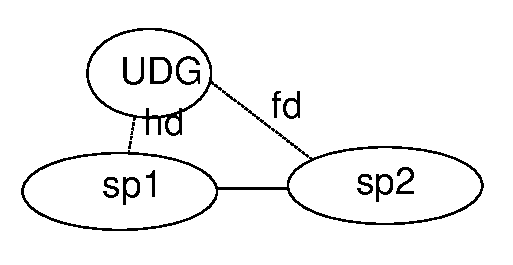
\includegraphics[width=1.0\textwidth]{ber/berintermediate}
  \caption[A $UDG$ unit whilst performing a step along a DNA strand.]{A $UDG$ unit whilst performing a step along a DNA strand. The $hd$ bond is broken together with the new $fd$ being formed.}
  \label{fig:berintermediate}
\end{figure}

We model the deoxyribose/phosphate groups first. This has two ends, normally called 3' and 5', which we model as $p3$ and $p5$ actions respectively. They help us to build the DNA strands. Also, there is a $b$ action, which enables binding of a base. Then we need a possibility for the UDG to bind and to ``walk'': this is enabled by actions $d$, $h$, and $f$, as we will see. UDG is modelled to have the prefix $(h;f)$, which enables the walk, since the strong action $h$ can be bonded to a $DP$ and $f$ can interact with a neighbouring $DP$. This breaks the $hd$ bond, and the $fd$ bond is then promoted to $d$, which gives us the $UDG$ being bonded to the neighbouring $DP$ the same way it was bound before to the other $DP$. Figure~\ref{fig:berintermediate} shows this intermediate situation whilst this step is performed. The five bases ($C$, $G$, $T$, $A$) all have a $b$ action to bind to a $DP$. If $A-T$ respectively $C-G$ are opposite each other they can bind and therefore form a correct base pair in the DNA. Uracil ($U$) is not able to form a base pair in our DNA context. All bases have a weak action in the prefix $(b;x)$. This action $x$ serves for removing the base from the DNA by breaking the $b$ bond. For uracil the action $x$ is $e$, for other bases it is $i$. By this UDG can be specific to uracil. In our model no action interacts with $i$, but of course other proteins not modelled might react with it. Note that $i$ and $e$ actions in the $U$, $A$, $T$, $G$, and $C$ processes cannot happen if the $u, a, t, g$ respctively $c$ actions are done, so $i$ and $e$ are blocked by $u, a, t, g,$ and $c$. Since $u, a, t, g$ and $c$ are used to form the base pairs this means that a correct base pair cannot be removed from the DNA in any case. This models the situation we need for the repair mechanism to work. We have used concerted actions in two instances here: Firstly to enable the UDG walk. This is an instance where backtracking would not work, since we need out-of-causal-order reversibility in this case. We cannot unbond from the old DP first and then choose the next $DP$, but we must hold the old bond until the new bond is formed. Secondly, we use a concerted action to enable the repair mechanism by making a bonding on the repair action break the bond to DP.

In the synchronisation function, we have the interaction of $p3$ and $p5$ to form the strands, the $b$-$b$ interaction for binding the bases, the $h$-$d$ and $f$-$d$ interaction for the ``walk'', the $a$-$t$ and $g$-$c$ interactions for forming the base pairs, and the $e$-$e$ interaction for the repair action.

In order to model a strand of DNA, we restrict ourselves to three base pairs. This means we need six $DP$ processes and six bases. We put two ``correct'' base pairs and one containing a uracil base. An extra $C$ base must be available for replacing $U$. We also use subscripts to distinguish processes where there is more than one instance of the process. The system is modelled in CCB as follows:

$$\begin{array}{l}
(DP_1 \paral DP_2 \paral DP_3 \paral A \paral T \paral G_1 \paral G_2 \paral U \paral C_1 \paral C_2 \paral DP_4 \paral DP_5 \paral DP_6 \paral UDG) \\
\setminus\{p3, p5, d, b, a, t, g, e, u, c, h, f, i\} 
\end{array}$$ 

We leave out the restriction from now on for ease of reading. We number actions using subscripts where there is more than one instance, and set initial bonds as required. We get the following process:
%
\begin{flalign*}
&(p3_1,p5_1[1],d_1,b_1[5]).DP_1' \paral (p3_2[1],p5_2[3],d_2,b_2[4]).DP_2' \paral (p3_3[3],p5_3,d_3,b_3[9]).DP_3' \paral &&\\
&(b_1[5];i_1).(a[6]).A' \paral (b_2[7];i_2).(t[6]).T' \paral (b_3[8];i_3).(g_1).G_1' \paral  ((b_4[9];i_4).(g_2[10]).G_2'  \paral &&\\
&(b_5[4];e_2).(u).U' \paral (b_6[11];i_6).(c_1[10]).C' \paral (b_7;i_7).(c_2).C' \paral (p3_4,p5_4[12],d_4,b_4[7]).DP_4' \paral &&\\ &(p3_5[12],p5_5[13],d_5,b_5[8]).DP_5' \paral (p3_6[13],p5_6,d_6,b_6[11]).DP_6' \paral (h;f).(e_2).UDG'&&
\end{flalign*}
%
\begin{figure}[h!]
\psfrag{UDG}{${\mathrm{UDG}}$}
\psfrag{sp1}{${\mathrm{DP_1}}$}
\psfrag{sp2}{${\mathrm{DP_2}}$}
\psfrag{sp3}{${\mathrm{DP_3}}$}
\psfrag{sp4}{${\mathrm{DP_4}}$}
\psfrag{sp5}{${\mathrm{DP_5}}$}
\psfrag{sp6}{${\mathrm{DP_6}}$}
\psfrag{A}{${\mathrm{A}}$}
\psfrag{T}{${\mathrm{T}}$}
\psfrag{C1}{${\mathrm{C_1}}$}
\psfrag{C2}{${\mathrm{C_2}}$}
\psfrag{G1}{${\mathrm{G_1}}$}
\psfrag{G2}{${\mathrm{G_2}}$}
\psfrag{U}{${\mathrm{U}}$}
\psfrag{1}{${\mathrm{1}}$}
\psfrag{2}{${\mathrm{2}}$}
  \centering
    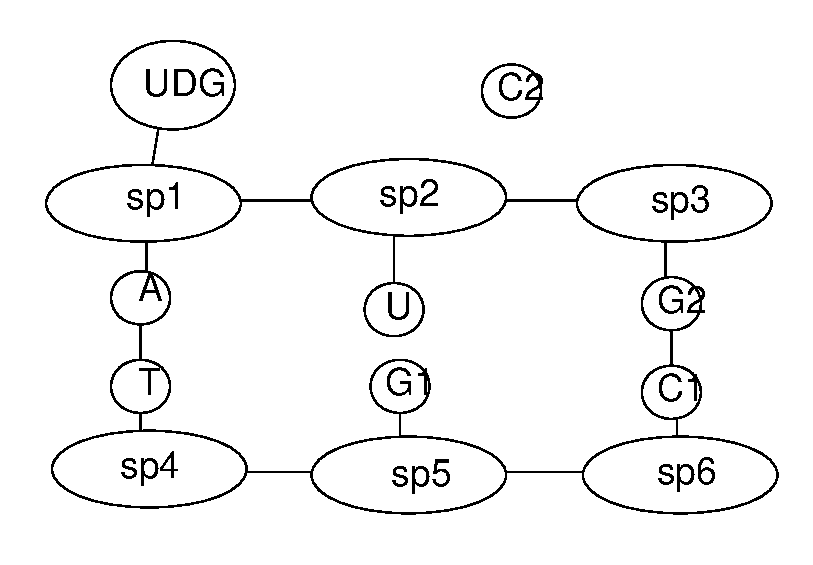
\includegraphics[width=1.0\textwidth]{ber/ber}
  \caption[A three base pair DNA fragment.]{A three base pair DNA fragment, with a uracil instead of a cytosine, and a UDG protein attached.}
  \label{fig:ber}
\end{figure}

Initially $UDG$ bonds to $DP_1$, which in turn is bonded to a correct base pair (note $UDG$ was not bound so far to any other process). The situation is shown in Figure~\ref{fig:ber} and is as follows (the bonds created, news keys and action on which keys were removed are shown in \textbf{bold}):
%
\begin{flalign*}
&\xrightarrow{hd[2]}(p3_1,p5_1[1],d_1\boldsymbol{[2]},b_1[5]).DP_1' \paral (p3_2[1],p5_2[3],d_2,b_2[4]).DP_2' \paral &&\\
&(p3_3[3],p5_3,d_3,b_3[9]).DP_3' \paral
(b_1[5];i_1).(a[6]).A' \paral (b_2[7];i_2).(t[6]).T' \paral (b_3[8];i_3).(g_1).G_1' \paral &&\\
&((b_4[9];i_4).(g_2[10]).G_2'  \paral (b_5[4];e_2).(u).U' \paral (b_6[11];i_6).(c_1[10]).C' \paral (b_7;i_7).(c_2).C' \paral &&\\
&(p3_4,p5_4[12],d_4,b_4[7]).DP_4' \paral (p3_5[12],p5_5[13],d_5,b_5[8]).DP_5' \paral &&\\
&(p3_6[13],p5_6,d_6,b_6[11]).DP_6' \paral (h\boldsymbol{[2]};f).(e_2).UDG'&&
\end{flalign*}
%
The UDG can now randomly ``walk'' along the chain. The $(h;f)$ prefix can appropriately model this, since if the weak $f$ action binds to the neighbour, the bond on $h$ is broken. In our case, action $f$ in $UDG$ can communicate with $d_2$ in $DP_2$. This breaks bond 2 from $h$ in $UDG$ to $d_1$ in $DP_1$, thus having performed a ``step''. We then move key $14$ from $f$ to $h$ (via the \rulename{prom} rule from Figure~\ref{fig:reduction}) and get:
%
\begin{flalign*}
&\xrightarrow{\{fd[14],\underline{hd}[2]\}} \Rightarrow (p3_1,p5_1[1],\boldsymbol{d_1},b_1[5]).DP_1' \paral (p3_2[1],p5_2[3],\boldsymbol{d_2[14]},b_2[4]).DP_2' \paral&&\\
&(p3_3[3],p5_3,d_3,b_3[9]).DP_3' \paral (b_1[5];i_1).(a[6]).A' \paral (b_2[7];i_2).(t[6]).T' \paral (b_3[8];i_3).(g_1).G_1' \paral&&\\
&((b_4[9];i_4).(g_2[10]).G_2'  \paral (b_5[4];e_2).(u).U' \paral (b_6[11];i_6).(c_1[10]).C' \paral (b_7;i_7).(c_2).C' \paral&&\\
&(p3_4,p5_4[12],d_4,b_4[7]).DP_4' \paral (p3_5[12],p5_5[13],d_5,b_5[8]).DP_5' \paral\\ &(p3_6[13],p5_6,d_6,b_6[11]).DP_6' \paral \boldsymbol{(h[14];f)}.(e_2).UDG'&&
\end{flalign*}
%
$UDG$ could now simply continue its walk, or it can interact via its $e$ action with the uracil. Note that other bases expose the $i$ action, so uracil cannot interact with them. The $u$, $a$, $t$, $g$, or $ c$ actions block $e$ or $i$, so correct base pairs are not affected by repairs. In our example $e_2$ on $UDG$ interacts with $e_2$ on $U$, breaking bond 4 between $b_5$ in $UDG$ and $b_2$ in $DP_2$. We have achieved the desired repair, since the uracil is removed from the DNA. We model this by the following transition (we use the rewrite rule again):
%
\begin{flalign*}
&\xrightarrow{\{ee[15],\underline{bb}[4]\}} \Rightarrow (p3_1,p5_1[1],d_1,b_1[5]).DP_1' \paral (p3_2[1],p5_2[3],d_2[14],\boldsymbol{b_2}).DP_2' \paral&&\\
&(p3_3[3],p5_3,d_3,b_3[9]).DP_3' \paral (b_1[5];i_1).(a[6]).A' \paral (b_2[7];i_2).(t[6]).T' \paral (b_3[8];i_3).(g_1).G_1' \paral&&\\
&((b_4[9];i_4).(g_2[10]).G_2'  \paral \boldsymbol{(b_5[15];e_2)}.(u).U' \paral (b_6[11];i_6).(c_1[10]).C' \paral (b_7;i_7).(c_2).C' \paral&&\\
&(p3_4,p5_4[12],d_4,b_4[7]).DP_4' \paral (p3_5[12],p5_5[13],d_5,b_5[8]).DP_5' \paral\\ &(p3_6[13],p5_6,d_6,b_6[11]).DP_6' \paral (h[14];f).(\boldsymbol{e_2[15]}).UDG'&&
\end{flalign*}
%
The floating $C_2$ can now take the place of the $U$ by binding to $DP_2$ and $G_1$. This is represented by the following two transitions:
%
\begin{flalign*}
&\xrightarrow{bb[16]}\xrightarrow{gc[17]}(p3_1,p5_1[1],d_1,b_1[5]).DP_1' \paral (p3_2[1],p5_2[3],d_2[14],\boldsymbol{b_2[16]}).DP_2' \paral&&\\
&(p3_3[3],p5_3,d_3,b_3[9]).DP_3' \paral (b_1[5];i_1).(a[6]).A' \paral (b_2[7];i_2).(t[6]).T' \paral (b_3[8];i_3).(\boldsymbol{g_1[17]}).G_1' \paral&&\\
&((b_4[9];i_4).(g_2[10]).G_2'  \paral (b_5[15];e_2).(u).U' \paral (b_6[11];i_6).(c_1[10]).C' \paral (\boldsymbol{b_7[16]};i_7).(\boldsymbol{c_2[17]}).C' \paral&&\\
&(p3_4,p5_4[12],d_4,b_4[7]).DP_4' \paral (p3_5[12],p5_5[13],d_5,b_5[8]).DP_5' \paral\\ &(p3_6[13],p5_6,d_6,b_6[11]).DP_6' \paral (h[14];f).(e_2[15]).UDG'&&
\end{flalign*}
%
The resulting process is shown in Figure~\ref{fig:ber2}.

\begin{figure}[h!]
\psfrag{UDG}{${\mathrm{UDG}}$}
\psfrag{sp1}{${\mathrm{DP_1}}$}
\psfrag{sp2}{${\mathrm{DP_2}}$}
\psfrag{sp3}{${\mathrm{DP_3}}$}
\psfrag{sp4}{${\mathrm{DP_4}}$}
\psfrag{sp5}{${\mathrm{DP_5}}$}
\psfrag{sp6}{${\mathrm{DP_6}}$}
\psfrag{A}{${\mathrm{A}}$}
\psfrag{T}{${\mathrm{T}}$}
\psfrag{C1}{${\mathrm{C_1}}$}
\psfrag{C2}{${\mathrm{C_2}}$}
\psfrag{G1}{${\mathrm{G_1}}$}
\psfrag{G2}{${\mathrm{G_2}}$}
\psfrag{U}{${\mathrm{U}}$}
\psfrag{1}{${\mathrm{1}}$}
\psfrag{2}{${\mathrm{2}}$}
  \centering
    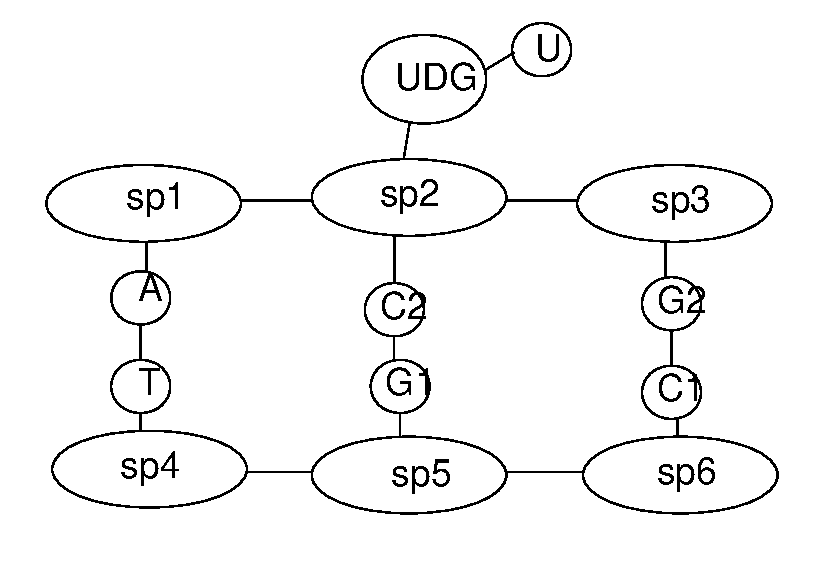
\includegraphics[width=1.0\textwidth]{ber/ber2}
  \caption[The repaired DNA fragment.]{The repaired DNA fragment, with the uracil replaced by a cytosine.}
  \label{fig:ber2}
\end{figure}

If uracil would have been bonded on $u$, the interaction with UDG could not have happened, so the defect is recognized. We now have the uracil broken from the deoxyribose/phosphate group and the $b$ action on the deoxyribose/phosphate group ready to bond to another base. UDG needs to release $U$ and then either to continue its walk or release itself from the DNA. We can again use our new operator for modelling UDG, since this way we achieve that the repair mechanism happens. On the other hand by combining two groups of actions we ``block'' this repair to happen if the desired second bond is there.

A limitation of our modelling is that it allows the UDG during its ``walk'' to bind to any DG group, since there is no restriction which $d$ action is used. In reality of course UDG must continue with the nearest DP group. This is a spatial effect our calculus does not model so far. Similarly, the repair by UDG binding to the $e$ action of a uracil (U) is not dependent on the UDG being next to it, whereas in reality it is. Again this is a spatial effect, which we will discuss in Section~\ref{sec:ccbs}.

We have used the software from Chapter~\ref{sec:simulation} to test the modelling. The desired path is one of the possibilities, which shows that our modelling is adequate in this respect. We also get some undesired reactions: Apart from UDG binding to any DP group during its walk, there is also the possibility that the unused $p5$ action of a $DP$, which is at the end of the DNA strand, interacts with an unused $p3$ from the a DP at the other end of the DNA strand. This is not impossible as a such, but prevented in reality by at least two effects we do not model. One is again the spatial arrangement, the other is the fact that the ends of the DNA are protected by special groups, which we do not model here. They prevent reactions at the DNA ends.

\section{DNA Mismatch Repair}
\label{sec:dnamimatch}

\subsection{Description of DNA Mismatch Repair}

In Section~\ref{sec:ber}, the problem was the incorporation into DNA of a base which should not occur in DNA at all. The repair relied on recognizing this base. Another possible error is that two bases are included which are both possible in DNA, but do not match, for example, a pair of adenine and cytosine. This can happen if, after the splitting of the double strand, the new strand intended to match the old one, does not actually match the old strand - for example, incorporating a adenine opposite a cytosine, which should normally be matched by a thymine.

Such a repair (a DNA mismatch repair, called MMR herafter) is not possible in the same way as the base excision repair, since any of the two bases could be wrong, so the non-matching  bases do not tell what to do.  As before, we model the process using several abstractions. A description of the process on an abstract level is as follows: If two bases are incorporated into a DNA strand which do not match (i.e. are not C/G or A/T pairs), this constitutes a defect in the DNA strand. A repair similar to the BER is not possible, since it is not clear which of the two bases is correct just from the bases alone - both could be right. We are looking at a specific way to handle this situation, called Methyl Mismatch Repair (MMR). This is the repair mechanism in bacteria, in particular E. coli, for which detailled studies has been done.\footnote{Paul L. Modrich, Tomas Lindahl and Aziz Sancar received the Nobel Price in Chemistry 2015 for their work on DNA repair. Modrich's Nobel Lecture about Methyl-directed Mismatch Repair in E. coli and humans \cite{pmid27198632} gives a nice overview.}, This process is based on DNA strands being methylated some time after their creation. Methylation means the attachment a methyl group (a carbon atom with three hydrogen atoms), in this case to the Adenine base. Specifically this happens whenever there is a GATC sequence. Since the methylation (which is done by specific proteins, which we do not model) happens with a delay after the duplication of a strand, for some time the old strand is methylated, the new strand is not. This enables the removal of specifially the new base, which must be the wrong one.

The actual repair involved the proteins MutS, MutL, MutH, and UvrD. MutS first binds to the mismatch and then recruits MutL and MutH. MutL can detected the methylated strand and can form a loop in the DNA. In this loop, the newer strand now is outside, whereas the old strand is covered by itself and MutL. MutH cleavs the unmethylated strand. This happens in some distance from the mismatch, due to the size of the proteins and the loop in the DNA. UvrD can then detect the cleavage and can move along the strand. It removes the outer strand when moving along. At the same time, the MutL, MutH, and MutS proteins are released and the loop in the DNA disappears. UvrD moves to after the mismatch, removing the wrong base together with their neighbours. UvrD then goes off the DNA and leaves the old, and correct, strand to be completed. 

\subsection{Modelling DNA Mismatch Repair}

For modelling MMR, we use the components from Section~\ref{sec:ber} as much as possiible. We reuse the deoxyribose/phosphate groups, and the four bases A, T, C, and G. We will extend those components where needed, but we will keep the original actions. Overall, in order to model MMR, we need the following components: deoxyribose/phosphate groups, the four bases A, T, G, C, the methyl group Me, and the proteins MutS, MutL, MutH, and UvrD. The resused components are the following:
%
$$\begin{array}{lll}
DP & \bydef & (p3,p5;s).DP' \paral (b,d).DP'\\
A & \bydef & (b;i).(a;r).(m).A'\\
T & \bydef & (b;i).(t;r).T'\\
G & \bydef & (b;i).(g;r).G'\\
C & \bydef & (b;i).(c;r).C'\\
\end{array}$$
%
where processes $A$, $T$, $G$, and $C$ model the bases adenine (A), cytosine (C), guanine (G), and thymine (T). Notice we have added actions s, m, and r. Also the actions on DP have been regrouped (but all original actions are still there). In DP, we are now using a parallel operator. This is necessary to enable a breaking of a bond to p3 or p5 whilst there is still a bond to $b$. The action $d$, which was used by UDG in the modelling of BER is not used here, as we will see. We keep it to have an extension of the previous modelling.

We also need additional components, namely the methyl group, the MutS, MutL, MutH, and UvrD proteins. We model these as follows:
$$\begin{array}{lll}
Me & \bydef & (m).(n).Me'\\
MS & \bydef & (m2,m2).(l).MS'\\
ML & \bydef & (l).(n).(o).ML'\\
MH & \bydef & (o).(w).MH'\\
UD & \bydef & (u;r).UD' \paral (v;s).UD'\\
\end{array}$$
%
where processes $MS$, $ML$, $MH$, and $UD$ model the MutS, MutL, MutH, and UvrD protein respectively.  Here $s$, $i$, and $r$ are weak actions, all other actions, namely $p3$, $p5$, $b$, $b$, $d$, $b$, $a$, $t$, $g$, $c$, m, n, m2, l, o, s, u, v and w are strong. Notice that $i$ is not used, but we keep it to have this model as an extension of the BER model. In UD, we again use a  parallel operator. This will make it possible for UvrD to break two bonds with every ``step'' it moves.


The synchronisation function for our system is as follows:
%
$$\begin{array}{ l c l l }
\gamma(p3,p5) & = & p & \\
\gamma(b,b) & = & bb &\\
\gamma(a,t) & = & at &  \\
\gamma(g,c) & = & gc & \\
\gamma(m,m) & = & mm & \\
\gamma(m2,a) & = & m2a & \\
\gamma(m2g) & = & m2g & \\
\gamma(m2c) & = & m2c & \\
\gamma(m2t) & = & m2t & \\
\gamma(l,l) & = & ll & \\
\gamma(n,n) & = & nn & \\
\gamma(o,o) & = & oo & \\
\gamma(r,r) & = & rr & \\
\gamma(t,u) & = & tu & \\
\gamma(p,s) & = & ps & \\
\gamma(w,s) & = & ws & \\
\end{array}$$

As before, the deoxyribose/phosphate groups and the bases can combine to form a DNA strand. In that strand, there can be DNA mismatches. Note that we do not model how they happen, we just assume a DNA strand as in Figure~\ref{fig:state1} with a DNA mismatch and correct pairs otherwise. The mismatch here is an A-G pair, but that is not crucial for our modelling. The A-G bases cannot bond to each other, that is the case in our modelling as well in reality, and this gives the opportunity for the repair. To the left of the DNA strand, there is a CTAG sequence (respectively a GATC sequence). This is where the methylation happens. In our case, we have a recently duplicated strand, where the older part is the upper one (A is methylated) and the newer part is the lower one (A is not methylated). The methylation itself is done by proteins which are not modelled here. This is the situation where the MMR can happen.

\begin{figure}[h!]
\psfrag{UDG}{${\mathrm{UDG}}$}
\psfrag{sp1}{${\mathrm{DP_1}}$}
\psfrag{sp2}{${\mathrm{DP_2}}$}
\psfrag{sp3}{${\mathrm{DP_3}}$}
\psfrag{sp4}{${\mathrm{DP_4}}$}
\psfrag{sp5}{${\mathrm{DP_5}}$}
\psfrag{sp6}{${\mathrm{DP_6}}$}
\psfrag{A}{${\mathrm{A}}$}
\psfrag{T}{${\mathrm{T}}$}
\psfrag{C1}{${\mathrm{C_1}}$}
\psfrag{C2}{${\mathrm{C_2}}$}
\psfrag{G1}{${\mathrm{G_1}}$}
\psfrag{G2}{${\mathrm{G_2}}$}
\psfrag{U}{${\mathrm{U}}$}
\psfrag{1}{${\mathrm{1}}$}
\psfrag{2}{${\mathrm{2}}$}
  \centering
    %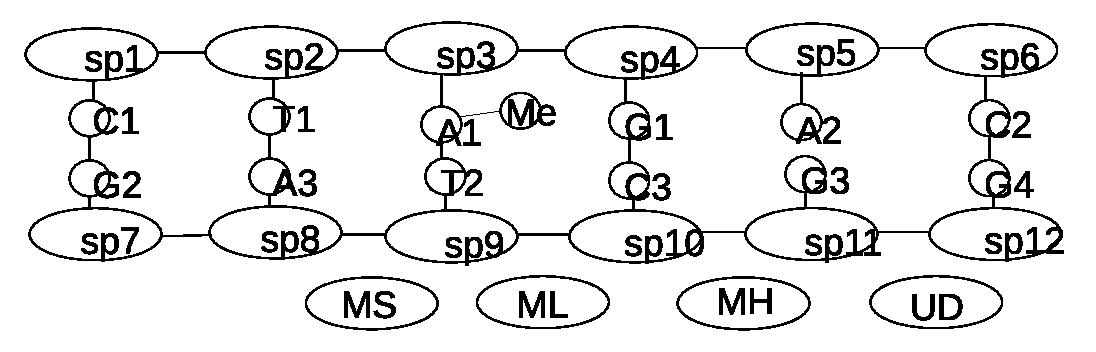
\includegraphics[width=1.0\textwidth]{mmr/state1}
  \caption[A six base pair DNA fragment.]{A six base pair DNA fragment, with a DNA mismatch and methylation of one strand. The proteins MutL, MutS, MutH, and UvrD are currently not bound to the DNA.}
  \label{fig:state1}
\end{figure}

We can model this similar to what we did before as:

$$\begin{array}{l}
(DP_1 \paral DP_2 \paral DP_3 \paral DP_4 \paral DP_5 \paral DP_6 \paral A_1 \paral A_2 \paral A_3 \paral T_1 \paral T_2 \paral G_1 \paral G_2 \paral G_3 \paral G_4\\
\paral U \paral C_1 \paral C_2 \paral C_3 \paral DP_4 \paral DP_5 \paral DP_6 \paral Me \paral MS \paral ML \paral MH \paral UD) \\
\setminus\{p3, p5, s, i, r, b, b, d, b, a, t, g, c, m, n, m2, l, o, s, u, v, w\} 
\end{array}$$ 

We leave out the restriction from now on for ease of reading. We number actions using subscripts where there is more than one instance, and set initial bonds as required. We get the following process:
%
\begin{flalign*}
&(p3_1,p5_1[1];s_1).DP_1' \paral (b_1[10],d_1).DP_1' \paral (p3_2[1],p5_2[2];s_2).DP_2' \paral (b_2[8],d_2).DP_2' \paral (p3_3[2],p5_3[3];s_3).DP_3' \paral (b_3[6],d_3).DP_3' \paral &&\\
&(p3_4[3],p5_4[4];s_4).DP_4' \paral (b_4[9],d_4).DP_4' \paral (p3_5[4],p5_5[5];s_5).DP_5' \paral (b_5[7],d_5).DP_5' \paral (p3_6[5],p5_6;s_6).DP_6' \paral (b_6[11],d_6)).DP_6' \paral  &&\\
&(b_1[6];i_1).(a_1[24]).(m_1[27];r).A_1' \paral (b_2[7];i_2).(a_2[26]).(m_2;r).A_2' \paral (b_3[18];i_3).(a_2[23]).(m_2;r).A_3' \paral &&\\
&(b_4[8];i_4).(t_1[23]:r_1).T_1' \paral (b_5[19];i_5).(t_2[24];r_2).T_2' \paral  (b_6[9];i_6).(g_1[25];r_3).G_1' \paral &&\\
&(b_7[17];i_7).(g_2[23];r_4).G_2' \paral (b_8[21];i_8).(g_2[26];r_4).G_3' \paral (b_9[22];i_9).(g_2[27];r_4).G_4' \paral&&\\
&(b_9[10];i_9).(c_1[23];r).C_1' \paral (b_{10}[11];i_{10}).(c_2[27];r).C_2' \paral (b_{11}[20];i_{11}).(c_3[25];r).C_3'  \paral&&\\
&(p3_7,p5_7[12];s_7).DP_7' \paral (b_7[17],d_7).DP_7' \paral (p3_8[12],p5_8[13];s_8).DP_8' \paral (b_8[18],d_8).DP_8' \paral (p3_9[13],p5_9[14];s_9).DP_9' \paral (b_9[19],d_9).DP_9' \paral &&\\
&(p3_{10}[14],p5_{10}[15];s_{10}).DP_{10}' \paral (b_{10}[20],d_{10})).DP_{10}' \paral  (p3_{11}[15],p5_{11}[16];s_{11}).DP_{11}' \paral (b_{11}[21],d_{11}).DP_{11}' \paral &&\\
&(p3_{12}[16],p5_{12};s_{12}).DP_{12}' \paral (b_{12}[22],d_{12}).DP_12' \paral  (m[27]).(n).Me'\paral (m2,m2).(l).MS' \paral (l).(n).(o).ML' \paral &&\\
&(o).(w).MH' \paral (u;r).UD' \paral (v;s).UD'&&
\end{flalign*}

MutS can now bond to the $A$ and $G$ bases via the $a$ and $g$ actions. This is the recognition of the mismatch. The bonding is not possible if the bases are properly paired, and also not if a Uracil is incorporated into the strand (as in the BER example). The transition for the bonding of MutS is as follows:

\begin{flalign*}
&\xrightarrow{\{m2a[28]\}} \xrightarrow{\{m2g[29]\}} (p3_1,p5_1[1];s_1).DP_1' \paral (b_1[10],d_1).DP_1' \paral (p3_2[1],p5_2[2];s_2).DP_2' \paral (b_2[8],d_2).DP_2' \paral (p3_3[2],p5_3[3];s_3).DP_3' \paral (b_3[6],d_3).DP_3' \paral &&\\
&(p3_4[3],p5_4[4];s_4).DP_4' \paral (b_4[9],d_4).DP_4' \paral (p3_5[4],p5_5[5];s_5).DP_5' \paral (b_5[7],d_5).DP_5' \paral (p3_6[5],p5_6;s_6).DP_6' \paral (b_6[11],d_6)).DP_6' \paral  &&\\
&(b_1[6];i_1).(a_1[24]).(m_1[27];r).A_1' \paral (b_2[7];i_2).(\mathbf{a_2[28]}).(m_2;r).A_2' \paral (b_3[18];i_3).(a_2[23]).(m_2;r).A_3' \paral &&\\
&(b_4[8];i_4).(t_1[23]:r_1).T_1' \paral (b_5[19];i_5).(t_2[24];r_2).T_2' \paral  (b_6[9];i_6).(g_1[25];r_3).G_1' \paral &&\\
&(b_7[17];i_7).(g_2[23];r_4).G_2' \paral (b_8[21];i_8).(\mathbf{g_2[29]};r_4).G_3' \paral (b_9[22];i_9).(g_2[27];r_4).G_4' \paral&&\\
&(b_9[10];i_9).(c_1[23];r).C_1' \paral (b_{10}[11];i_{10}).(c_2[27];r).C_2' \paral (b_{11}[20];i_{11}).(c_3[25];r).C_3'  \paral&&\\
&(p3_7,p5_7[12];s_7).DP_7' \paral (b_7[17],d_7).DP_7' \paral (p3_8[12],p5_8[13];s_8).DP_8' \paral (b_8[18],d_8).DP_8' \paral (p3_9[13],p5_9[14];s_9).DP_9' \paral (b_9[19],d_9).DP_9' \paral &&\\
&(p3_{10}[14],p5_{10}[15];s_{10}).DP' \paral (b_{10}[20],d_{10})).DP_{10}' \paral  (p3_{11}[15],p5_{11}[16];s_{11}).DP_{11}' \paral (b_{11}[21],d_{11}).DP_{11}' \paral &&\\
&(p3_{12}[16],p5_{12};s_{12}).DP_{12}' \paral (b_{12}[22],d_{12}).DP_12' \paral  (m[27]).(n).Me'\paral (\mathbf{m2[28],m2[29]}).(l).MS' \paral (l).(n).(o).ML' \paral &&\\
&(o).(w).MH' \paral (u;r).UD' \paral (v;s).UD'&&
\end{flalign*}

Now it is possible for MutL to bond to MutS:

\begin{flalign*}
&\xrightarrow{\{ll[30]\}} (p3_1,p5_1[1];s_1).DP_1' \paral (b_1[10],d_1).DP_1' \paral (p3_2[1],p5_2[2];s_2).DP_2' \paral (b_2[8],d_2).DP_2' \paral (p3_3[2],p5_3[3];s_3).DP_3' \paral (b_3[6],d_3).DP_3' \paral &&\\
&(p3_4[3],p5_4[4];s_4).DP_4' \paral (b_4[9],d_4).DP_4' \paral (p3_5[4],p5_5[5];s_5).DP_5' \paral (b_5[7],d_5).DP_5' \paral (p3_6[5],p5_6;s_6).DP_6' \paral (b_6[11],d_6)).DP_6' \paral  &&\\
&(b_1[6];i_1).(a_1[24]).(m_1[27];r).A_1' \paral (b_2[7];i_2).(a_2[28]).(m_2;r).A_2' \paral (b_3[18];i_3).(a_2[23]).(m_2;r).A_3' \paral &&\\
&(b_4[8];i_4).(t_1[23]:r_1).T_1' \paral (b_5[19];i_5).(t_2[24];r_2).T_2' \paral  (b_6[9];i_6).(g_1[25];r_3).G_1' \paral &&\\
&(b_7[17];i_7).(g_2[23];r_4).G_2' \paral (b_8[21];i_8).(g_2[29];r_4).G_3' \paral (b_9[22];i_9).(g_2[27];r_4).G_4' \paral&&\\
&(b_9[10];i_9).(c_1[23];r).C_1' \paral (b_{10}[11];i_{10}).(c_2[27];r).C_2' \paral (b_{11}[20];i_{11}).(c_3[25];r).C_3'  \paral&&\\
&(p3_7,p5_7[12];s_7).DP'_7 \paral (b_7[17],d_7).DP_7' \paral (p3_8[12],p5_8[13];s_8).DP_8' \paral (b_8[18],d_8).DP_8' \paral (p3_9[13],p5_9[14];s_9).DP_9' \paral (b_9[19],d_9).DP_9' \paral &&\\
&(p3_{10}[14],p5_{10}[15];s_{10}).DP_{10}' \paral (b_{10}[20],d_{10})).DP_{10}' \paral  (p3_{11}[15],p5_{11}[16];s_{11}).DP_{11}' \paral (b_{11}[21],d_{11}).DP_{11}' \paral &&\\
&(p3_{12}[16],p5_{12};s_{12}).DP_{12}' \paral (b_{12}[22],d_{12}).DP_12' \paral  (m[27]).(n).Me'\paral (m2[28],m2[29]).(\mathbf{l[30]}).MS' \paral (\mathbf{l[30]}).(n).(o).ML' \paral &&\\
&(o).(w).MH' \paral (u;r).UD' \paral (v;s).UD'&&
\end{flalign*}

MutL now can bond with Me, which means it detects which of the strands is methylated, and therefore the correct one:

\begin{flalign*}
&\xrightarrow{\{nn[31]\}} (p3_1,p5_1[1];s_1).DP-1' \paral (b_1[10],d_1).DP_1' \paral (p3_2[1],p5_2[2];s_2).DP_2' \paral (b_2[8],d_2).DP_2' \paral (p3_3[2],p5_3[3];s_3).DP_3' \paral (b_3[6],d_3).DP_3' \paral &&\\
&(p3_4[3],p5_4[4];s_4).DP_4' \paral (b_4[9],d_4).DP_4' \paral (p3_5[4],p5_5[5];s_5).DP_5' \paral (b_5[7],d_5).DP_5' \paral (p3_6[5],p5_6;s_6).DP_6' \paral (b_6[11],d_6)).DP_6' \paral  &&\\
&(b_1[6];i_1).(a_1[24]).(m_1[27];r).A_1' \paral (b_2[7];i_2).(a_2[28]).(m_2;r).A_2' \paral (b_3[18];i_3).(a_2[23]).(m_2;r).A_3' \paral &&\\
&(b_4[8];i_4).(t_1[23]:r_1).T_1' \paral (b_5[19];i_5).(t_2[24];r_2).T_2' \paral  (b_6[9];i_6).(g_1[25];r_3).G_1' \paral &&\\
&(b_7[17];i_7).(g_2[23];r_4).G_2' \paral (b_8[21];i_8).(g_2[29];r_4).G_3' \paral (b_9[22];i_9).(g_2[27];r_4).G_4' \paral&&\\
&(b_9[10];i_9).(c_1[23];r).C_1' \paral (b_{10}[11];i_{10}).(c_2[27];r).C_2' \paral (b_{11}[20];i_{11}).(c_3[25];r).C_3'  \paral&&\\
&(p3_7,p5_7[12];s_7).DP_7' \paral (b_7[17],d_7).DP_7' \paral (p3_8[12],p5_8[13];s_8).DP_8' \paral (b_8[18],d_8).DP_8' \paral (p3_9[13],p5_9[14];s_9).DP_9' \paral (b_9[19],d_9).DP_9' \paral &&\\
&(p3_{10}[14],p5_{10}[15];s_{10}).DP_{10}' \paral (b_{10}[20],d_{10})).DP_{10}' \paral  (p3_{11}[15],p5_{11}[16];s_{11}).DP_{11}' \paral (b_{11}[21],d_{11}).DP_{11}' \paral &&\\
&(p3_{12}[16],p5_{12};s_{12}).DP_{12}' \paral (b_{12}[22],d_{12}).DP_{12}' \paral  (m[27]).(\mathbf{n[31]}).Me'\paral (m2[28],m2[29]).(l[30]).MS' \paral (l[30]).(\mathbf{n[31]}).(o).ML' \paral &&\\
&(o).(w).MH' \paral (u;r).UD' \paral (v;s).UD'&&
\end{flalign*}

MutL is now ready to recruit MutH:

\begin{flalign*}
&\xrightarrow{\{oo[32]\}} (p3_1,p5_1[1];s_1).DP_1' \paral (b_1[10],d_1).DP_1' \paral (p3_2[1],p5_2[2];s_2).DP_2' \paral (b_2[8],d_2).DP_2' \paral (p3_3[2],p5_3[3];s_3).DP_3' \paral (b_3[6],d_3).DP_3' \paral &&\\
&(p3_4[3],p5_4[4];s_4).DP_4' \paral (b_4[9],d_4).DP_4' \paral (p3_5[4],p5_5[5];s_5).DP_5' \paral (b_5[7],d_5).DP_5' \paral (p3_6[5],p5_6;s_6).DP_6' \paral (b_6[11],d_6)).DP_6' \paral  &&\\
&(b_1[6];i_1).(a_1[24]).(m_1[27];r).A_1' \paral (b_2[7];i_2).(a_2[28]).(m_2;r).A_2' \paral (b_3[18];i_3).(a_2[23]).(m_2;r).A_3' \paral &&\\
&(b_4[8];i_4).(t_1[23]:r_1).T_1' \paral (b_5[19];i_5).(t_2[24];r_2).T_2' \paral  (b_6[9];i_6).(g_1[25];r_3).G_1' \paral &&\\
&(b_7[17];i_7).(g_2[23];r_4).G_2' \paral (b_8[21];i_8).(g_2[29];r_4).G_3' \paral (b_9[22];i_9).(g_2[27];r_4).G_4' \paral&&\\
&(b_9[10];i_9).(c_1[23];r).C_1' \paral (b_{10}[11];i_{10}).(c_2[27];r).C_2' \paral (b_{11}[20];i_{11}).(c_3[25];r).C_3'  \paral&&\\
&(p3_7,p5_7[12];s_7).DP_7' \paral (b_7[17],d_7).DP_7' \paral (p3_8[12],p5_8[13];s_8).DP_8' \paral (b_8[18],d_8).DP_8' \paral (p3_9[13],p5_9[14];s_9).DP_9' \paral (b_9[19],d_9).DP_9' \paral &&\\
&(p3_{10}[14],p5_{10}[15];s_{10}).DP_{10}' \paral (b_{10}[20],d_{10})).DP_{10}' \paral  (p3_{11}[15],p5_{11}[16];s_{11}).DP_{11}' \paral (b_{11}[21],d_{11}).DP_{11}' \paral &&\\
&(p3_{12}[16],p5_{12};s_{12}).DP_{12}' \paral (b_{12}[22],d_{12}).DP_12' \paral  (m[27]).(n[31]).Me'\paral (m2[28],m2[29]).(l[30]).MS' \paral (l[30]).(n[31]).(\mathbf{o[32]}).ML' \paral &&\\
&(\mathbf{o[32]}).(w).MH' \paral (u;r).UD' \paral (v;s).UD'&&
\end{flalign*}

MutH is now ready to cleave the DNA at the right location:

\begin{flalign*}
&\xrightarrow{\{ws[33],\underline{p5p3}[13]\}} \Rightarrow (p3_1,p5_1[1];s_1).DP_1' \paral (b_1[10],d_1).DP_1' \paral (p3_2[1],p5_2[2];s_2).DP_2' \paral (b_2[8],d_2).DP_2' \paral (p3_3[2],p5_3[3];s_3).DP_3' \paral (b_3[6],d_3).DP_3' \paral &&\\
&(p3_4[3],p5_4[4];s_4).DP_4' \paral (b_4[9],d_4).DP_4' \paral (p3_5[4],p5_5[5];s_5).DP_5' \paral (b_5[7],d_5).DP_5' \paral (p3_6[5],p5_6;s_6).DP_6' \paral (b_6[11],d_6)).DP_6' \paral  &&\\
&(b_1[6];i_1).(a_1[24]).(m_1[27];r).A_1' \paral (b_2[7];i_2).(a_2[28]).(m_2;r).A_2' \paral (b_3[18];i_3).(a_2[23]).(m_2;r).A_3' \paral &&\\
&(b_4[8];i_4).(t_1[23]:r_1).T_1' \paral (b_5[19];i_5).(t_2[24];r_2).T_2' \paral  (b_6[9];i_6).(g_1[25];r_3).G_1' \paral &&\\
&(b_7[17];i_7).(g_2[23];r_4).G_2' \paral (b_8[21];i_8).(g_2[29];r_4).G_3' \paral (b_9[22];i_9).(g_2[27];r_4).G_4' \paral&&\\
&(b_9[10];i_9).(c_1[23];r).C_1' \paral (b_{10}[11];i_{10}).(c_2[27]).C_2' \paral (b_{11}[20];i_{11}).(c_3[25];r).C_3'  \paral&&\\
&(p3_7,p5_7[12];s_7).DP_7' \paral (b_7[17],d_7).DP_7' \paral (p3_8[12],\mathbf{p5_8[33]};s_8).DP_8' \paral (b_8[18],d_8).DP_8' \paral (\mathbf{p3_9},p5_9[14];s_9).DP_9' \paral (b_9[19],d_9).DP_9' \paral &&\\
&(p3_{10}[14],p5_{10}[15];s_{10}).DP_{10}' \paral (b_{10}[20],d_{10})).DP_{10}' \paral  (p3_{11}[15],p5_{11}[16];s_{11}).DP_{11}' \paral (b_{11}[21],d_{11}).DP_{11}' \paral &&\\
&(p3_{12}[16],p5_{12};s_{12}).DP_{12}' \paral (b_{12}[22],d_{12}).DP_12' \paral  (m[27]).(n[31]).Me'\paral (m2[28],m2[29]).(l[30]).MS' \paral (l[30]).(n[31]).(o[32]).ML' \paral &&\\
&(o[32]).(\mathbf{w[33]}).MH' \paral (u;r).UD' \paral (v;s).UD'&&
\end{flalign*}

Note that execution of c on $DP_9$ leads to breaking a bond between two deoxyribose/phosphate groups. We use a concerted action and rewriting for this. The situation after this step is shown in Figure~\ref{fig:state2}. This has now the right DNA strand cleaved with the UvrD protein bonded to a DP group as well as a base.

\begin{figure}[h!]
\psfrag{UDG}{${\mathrm{UDG}}$}
\psfrag{sp1}{${\mathrm{DP_1}}$}
\psfrag{sp2}{${\mathrm{DP_2}}$}
\psfrag{sp3}{${\mathrm{DP_3}}$}
\psfrag{sp4}{${\mathrm{DP_4}}$}
\psfrag{sp5}{${\mathrm{DP_5}}$}
\psfrag{sp6}{${\mathrm{DP_6}}$}
\psfrag{A}{${\mathrm{A}}$}
\psfrag{T}{${\mathrm{T}}$}
\psfrag{C1}{${\mathrm{C_1}}$}
\psfrag{C2}{${\mathrm{C_2}}$}
\psfrag{G1}{${\mathrm{G_1}}$}
\psfrag{G2}{${\mathrm{G_2}}$}
\psfrag{U}{${\mathrm{U}}$}
\psfrag{1}{${\mathrm{1}}$}
\psfrag{2}{${\mathrm{2}}$}
  \centering
    \includegraphics[width=1.0\textwidth]{mmr/state2}
  \caption[A six base pair DNA fragment.]{A six base pair DNA fragment, with a DNA mismatch and methylation of one strand. TODO}
  \label{fig:state2}
\end{figure}

 Now the UvrD protein can use the cleavage to remove pairs of deoxyribose/phosphate groups and bases. This works as follows:

\begin{flalign*}
&\xrightarrow{\{sp3[34],\underline{at}[14]\}} \Rightarrow \xrightarrow{\{rr[35],\underline{at}[24]\}} \Rightarrow (p3_1,p5_1[1];s_1).DP_1' \paral (b_1[10],d_1).DP_1' \paral (p3_2[1],p5_2[2];s_2).DP_2' \paral (b_2[8],d_2).DP_2' \paral (p3_3[2],p5_3[3];s_3).DP_3' \paral (b_3[6],d_3).DP_3' \paral &&\\
&(p3_4[3],p5_4[4];s_4).DP_4' \paral (b_4[9],d_4).DP_4' \paral (p3_5[4],p5_5[5];s_5).DP_5' \paral (b_5[7],d_5).DP_5' \paral (p3_6[5],p5_6;s_6).DP_6' \paral (b_6[11],d_6)).DP_6' \paral  &&\\
&(b_1[6];i_1).(\mathbf{a_1}).(m_1[27];r).A_1' \paral (b_2[7];i_2).(a_2[28]).(m_2;r).A_2' \paral (b_3[18];i_3).(a_2[23]).(m_2;r).A_3' \paral &&\\
&(b_4[8];i_4).(t_1[23]:r_1).T_1' \paral (b_5[19];i_5).(\mathbf{t_2[35]};r_2).T_2' \paral  (b_6[9];i_6).(g_1[25];r_3).G_1' \paral &&\\
&(b_7[17];i_7).(g_2[23];r_4).G_2' \paral (b_8[21];i_8).(g_2[29];r_4).G_3' \paral (b_9[22];i_9).(g_2[27];r_4).G_4' \paral&&\\
&(b_9[10];i_9).(c_1[23];r).C_1' \paral (b_{10}[11];i_{10}).(c_2[27]).C_2' \paral (b_{11}[20];i_{11}).(c_3[25];r).C_3'  \paral&&\\
&(p3_7,p5_7[12];s_7).DP_7' \paral (b_7[17],d_7).DP_7' \paral (p3_8[12],p5_8[13];s_8).DP_8' \paral (b_8[18],d_8).DP_8' \paral (p3_9[13],p5_9[33];s_9).DP_9' \paral (b_9[19],d_9).DP_9' \paral &&\\
&(\mathbf{p3_{10}[34]},p5_{10}[15];s_{10}[11]).DP_{10}' \paral (b_{10}[20],d_{10})).DP_{10}' \paral  (\mathbf{p3_{11}[15]},p5_{11}[16];s_{11}).DP_{11}' \paral (b_{11}[21],d_{11}).DP_{11}' \paral &&\\
&(p3_{12}[16],p5_{12};s_{12}).DP_{12}' \paral (b_{12}[22],d_{12}).DP_12' \paral  (m[27]).(n[31]).Me'\paral (m2[28],m2[29]).(l[30]).MS' \paral (l[30]).(n[31]).(o[32]).ML' \paral &&\\
&(o[32]).(w[33]).MH' \paral (\mathbf{u35]};r).UD' \paral (\mathbf{v[34]};s).UD'&&
\end{flalign*}

From here, UvrD can ``walk'' along the strand. As opposed to BER, the bonds between the base pairs are now broken. In parallel, the bonds between the deoxyribose/phosphate groups are also broken as UvrD progresses:

\begin{flalign*}
&\xrightarrow{\{ss[36],\underline{p5p3}[15]\}} \Rightarrow \xrightarrow{\{rr[37],\underline{cg}[25]\}} \Rightarrow (p3_1,p5_1[1];s_1).DP_1' \paral (b_1[10],d_1).DP_1' \paral (p3_2[1],p5_2[2];s_2).DP_2' \paral (b_2[8],d_2).DP_2' \paral (p3_3[2],p5_3[3];s_3).DP_3' \paral (b_3[6],d_3).DP_3' \paral &&\\
&(p3_4[3],p5_4[4];s_4).DP_4' \paral (b_4[9],d_4).DP_4' \paral (p3_5[4],p5_5[5];s_5).DP_5' \paral (b_5[7],d_5).DP_5' \paral (p3_6[5],p5_6;s_6).DP_6' \paral (b_6[11],d_6)).DP_6' \paral  &&\\
&(b_1[6];i_1).(a_1).(m_1[27];r).A_1' \paral (b_2[7];i_2).(a_2[28]).(m_2;r).A_2' \paral (b_3[18];i_3).(a_2[23]).(m_2;r).A_3' \paral &&\\
&(b_4[8];i_4).(t_1[23]:r_1).T_1' \paral (b_5[19];i_5).(t_2[35];r_2).T_2' \paral  (b_6[9];i_6).(\mathbf{g_1};r_3).G_1' \paral &&\\
&(b_7[17];i_7).(g_2[23];r_4).G_2' \paral (b_8[21];i_8).(g_2[29];r_4).G_3' \paral (b_9[22];i_9).(g_2[27];r_4).G_4' \paral&&\\
&(b_9[10];i_9).(c_1[23];r).C_1' \paral (b_{10}[11];i_{10}).(c_2[27]).C_2' \paral (b_{11}[20];i_{11}).(\mathbf{c_3[37]};r).C_3'  \paral&&\\
&(p3_7,p5_7[12];s_7).DP_7' \paral (b_7[17],d_7).DP_7' \paral (p3_8[12],p5_8[13];s_8).DP_8' \paral (b_8[18],d_8).DP_8' \paral (p3_9[13],p5_9[33];s_9).DP_9' \paral (b_9[19],d_9).DP_9' \paral &&\\
&(p3_{10}[34],\mathbf{p5_{10}};s_{10}[11]).DP_{10}' \paral (b_{10}[20],d_{10})).DP_{10}' \paral  (\mathbf{p3_{11}[36]},p5_{11}[16];s_{11}).DP_{11}' \paral (b_{11}[21],d_{11}).DP_{11}' \paral &&\\
&(p3_{12}[16],p5_{12};s_{12}).DP_{12}' \paral (b_{12}[22],d_{12}).DP_12' \paral  (m[27]).(n[31]).Me'\paral (m2[28],m2[29]).(l[30]).MS' \paral (l[30]).(n[31]).(o[32]).ML' \paral &&\\
&(o[32]).(w[33]).MH' \paral (\mathbf{u37]};r).UD' \paral (\mathbf{v[36]};s).UD'&&
\end{flalign*}

This is shown in Figure~\ref{fig:state3}. This process can continue until the offending base has been removed. The protein complex can then unbond from the DNA and the exposed half-strand can be completed by the appropriate bases binding to them.

\begin{figure}[h!]
\psfrag{UDG}{${\mathrm{UDG}}$}
\psfrag{sp1}{${\mathrm{DP_1}}$}
\psfrag{sp2}{${\mathrm{DP_2}}$}
\psfrag{sp3}{${\mathrm{DP_3}}$}
\psfrag{sp4}{${\mathrm{DP_4}}$}
\psfrag{sp5}{${\mathrm{DP_5}}$}
\psfrag{sp6}{${\mathrm{DP_6}}$}
\psfrag{A}{${\mathrm{A}}$}
\psfrag{T}{${\mathrm{T}}$}
\psfrag{C1}{${\mathrm{C_1}}$}
\psfrag{C2}{${\mathrm{C_2}}$}
\psfrag{G1}{${\mathrm{G_1}}$}
\psfrag{G2}{${\mathrm{G_2}}$}
\psfrag{U}{${\mathrm{U}}$}
\psfrag{1}{${\mathrm{1}}$}
\psfrag{2}{${\mathrm{2}}$}
  \centering
    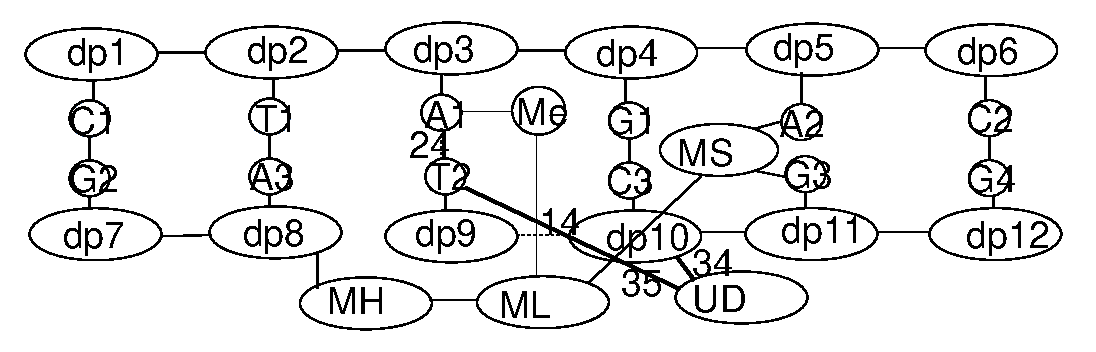
\includegraphics[width=1.0\textwidth]{mmr/state3}
  \caption[A six base pair DNA fragment.]{A six base pair DNA fragment, with a DNA mismatch and methylation of one strand. TODO}
  \label{fig:state3}
\end{figure}

\section{Related Work}

\section{Future Work}

\section{Conclusion}

\section*{References}

\bibliography{mybibfile}

\end{document}